\documentclass[a4paper,twoside,12pt]{report}

% Load packages
\usepackage[utf8x]{inputenc}
\usepackage[UKenglish]{babel}
\usepackage[round]{natbib}             % commands \citep e \citet for natural citations
\usepackage{nextpage}                  % blank pages with \cleartooddpage
\usepackage{amssymb}                   % maths stuff
\usepackage{amsfonts}                  % maths stuff
\usepackage{amsmath}                   % maths stuff
\usepackage{amsbsy}                    % maths stuff
\usepackage{color}                     % for coloured text & links
\usepackage{array,arydshln}
\usepackage{booktabs}                  % hrule with different widths and thicknesses
\usepackage{multirow}
\usepackage{pifont}
\usepackage{textcomp}
\usepackage[plain,chapter]{algorithm}  % for the algorithm environment
\usepackage{algpseudocode}             % for the algorithm pseudocode
\usepackage{setspace}                  % command \setstretch for line spacing on the text only
\usepackage[figuresright]{rotating}    % environment sidewaystable

% Temporary packages for testing
\usepackage{graphicx}              % comment this out with XeLaTeX, but keep with pdfLaTeX
% \usepackage{lipsum}                % Lorem ipsum

% Use XeLaTeX and set fonts
\usepackage{mathspec}           % keep math standard TeX fonts, not XeTeX fonts
\usepackage{xltxtra}            % for the XeLaTeX stuff (it incorporates fontspec)
\defaultfontfeatures{Mapping=tex-text,Contextuals=Swash,Ligatures={Required,Common,Contextual,Rare}}
\setmainfont[Numbers=Lining]{Linux Libertine O}
\setromanfont[Numbers=Lining]{Linux Libertine O}
\setsansfont{Linux Biolinum O}
\setmonofont[Scale=MatchLowercase]{Linux Mono O}
\renewcommand{\thepage}{\arabic{page}} % font for the page numbers as lining

% Format for the captions
\usepackage[labelfont=bf,font=small]{caption}
% \usepackage[bf,small,sf]{caption}

% Some colors
\definecolor{corlink}{rgb}{0, 0, .4}
\definecolor{orange}{rgb}{.7, .40, 0}

% Hyperlinks setup and meta-information
\usepackage{hyperref}
\hypersetup{
  colorlinks,
  citecolor   = corlink,
  filecolor   = corlink,
  linkcolor   = corlink,
  urlcolor    = corlink,
  pdftitle    = {New Strategies for Permutation Methods in Brain Imaging},
  pdfauthor   = {Anderson M. Winkler}}

% Header and footer
\usepackage{fancyhdr}
\usepackage[fit]{truncate}
\fancyhead[RE]{\truncate{0.9\headwidth}{\small\nouppercase{\textbf{\leftmark}}}}
\fancyhead[LO]{\truncate{0.9\headwidth}{\small\nouppercase{\textbf{\rightmark}}}}
\fancyhead[RO,LE]{\small\arabic{page}}  % right odd, left even
\fancyfoot{}
% \fancyfoot[C]{\textcolor{red}{\textbf{--- UNCORRECTED PROOF ---}}}

% Margins (this uses fancyhdr package)
%\usepackage{showframe}
\topmargin      = 0mm
\oddsidemargin  = 16mm % 5mm
\evensidemargin = 4mm  % 5mm
\marginparsep   = 0mm
\marginparwidth = 0mm
\textwidth      = 140mm
\textheight     = 225mm
\headwidth      = 140mm
\headheight     = 6mm

% Adjust footnotes indentation
\usepackage[hang,flushmargin]{footmisc} 
\renewcommand{\footnotemargin}{.8em}

% Other new commands
\newcommand{\ud}{\mathrm{d}}
\newcommand{\blankpage}{\cleartooddpage[\thispagestyle{empty}]}
\newcommand{\HRule}{\rule{\linewidth}{0.08em}}
\renewcommand\multirowsetup{\centering}

% Line spacing
%\linespread{1.35} % this affects everything
\newcommand{\lspac}{1.5}  % this affects only the main text, not footnotes, captions or tables
\setlength{\skip\footins}{10mm} % distance between text and footnotes
\setlength{\footnotesep}{4mm} % distance between the actual footnotes

% Sections up to level 4
\setcounter{secnumdepth}{3}
\setcounter{tocdepth}{3}

% For the title page
\title{New Strategies for Permutation Methods in Brain Imaging}
\author{Anderson M. Winkler}

\begin{document}
\maketitle
\bibliographystyle{scabbrvnat}

\pagestyle{fancy}
\setstretch{\lspac}
\blankpage \tableofcontents
\blankpage \listoffigures
\blankpage \listoftables
\blankpage \listofalgorithms
\setstretch{1}
\blankpage \chapter{Introduction}
\setstretch{\lspac}

The previous chapter discussed how permutation methods, for being free of various assumptions related to classical parametric tests, could better adapt to the growing variety of experimental imaging methods. In this chapter, these ideas are further extended to non-parametrically allow \emph{joint inference} on more than one modality, that is, how to infer about hypotheses concerning these modalities when more than one image is available for each subject. Examples of such modalities include the same cited in Chapter~\ref{sec:perm:permglm}, such as, but not limited to, positron emission tomography (\textsc{pet}), functional magnetic resonance imaging (\textsc{fmri}), tensor-based morphometry (\textsc{tbm}), diffusion tensor imaging (\textsc{dti}), cortical thickness and surface area, cerebral perfusion, as well as various others.

Further to these examples, it is also the case that the same imaging modality is often subdivided so as to better characterise certain physical properties --- including morphology and function --- of the biological tissue. As an example, diffusion-weighted images are often used to generate maps of fractional anisotropy (\textsc{fa}), mean diffusivity (\textsc{md}), radial diffusivity (\textsc{rd}), as well as lengths of the eigenvectors of the diffusion tensor and other measurements. Another example is the use of independent component analysis (\textsc{ica}) to decompose \textsc{fmri} time series into a set of timecourses and spatial maps. Only some of these components might be of actual interest, or the effect of interest might be split into more than one; in either case, a strategy that could combine the information from these into a single inferential step tends to be more meaningful than various separate tests. \citep{Fisher1932}
\blankpage \chapter{Permutation inference for the general linear model}
\label{sec:permglm}
\setstretch{\lspac}

\section{Introduction}

Neuroimaging research has continuously been expanded to encompass an ever growing variety of experimental methods. From the early experiments using positron emission tomography (\textsc{pet}) and functional magnetic resonance imaging (\textsc{fmri}), it is now often of interest to verify hypotheses using information obtained from, e.g.\ tensor-based morphometry (\textsc{tbm}), diffusion tensor imaging (\textsc{dti}), cortical thickness and surface area, cerebral perfusion, as well as many others and variations and combinations of these. All these different modalities produce images that have different physical and biological properties, as well as different information content. Despite this variety, most of the strategies for statistical analysis constitute linear models, and can be formulated within the \emph{general linear model} (\textsc{glm}). The \textsc{glm} is a simple, yet flexible framework of which many different types of analysis are particular cases \citep{Searle1971, Christensen2002}. The common strategy is to construct a plausible explanatory model for the observed data, estimate the parameters of this model, and compute a suitable statistic for testing of hypotheses on some or all of these parameters. The rejection or acceptance of a given hypothesis depends on the probablility of finding, due to chance alone, a statistic at least as high as the observed. Typically, but not necessarily, the hypothesis being tested is that one or more parameters are zero, being referred to as the \emph{null hypothesis}.

If the parameters of the distribution of the statistic under the hypothesis being tested, be it the null or not, is known, such probability can be ascertained using this distribution. In many particular cases, a mathematical expression describes the behaviour of the statistic as a function of these parameters, and this analytical representation of the distribution can be used for hypotheses testing as long as the data satisfies a certain set of requirements under which the distribution arises and can be recovered asymptotically. A conclusion based on these \emph{parametric tests} will only be sound as long as the observed data possess these assumed stochastic properties, even if other methodological aspects are valid. Strategies that may be used when these assumptions are not met include, among others, the use of \emph{non-parametric tests}.

\emph{Permutation methods}, sometimes also called \emph{randomisation} or \emph{re-randomisation} methods\footnote{See \citet{Nichols2002} for distinct usage of these terms accoding to the justification for data exchangeability.} are a class of these non-parametric methods. They were pioneered by \citet{Fisher1935} and \citet{Pitman1937-I, Pitman1937-II, Pitman1938}. Fisher demonstrated that the null hypothesis could be tested simply by observing, after permuting observations, how often the difference between means would exceed the difference found without permutation, and that for such test, no normality would be required, differently therefore than most parametric tests.\footnote{Although Fisher pioneered the idea of permuting observations once an experiment had been performed, the idea of actually repeating the same experiment many times, with the experimental conditions being permuted to determine significances, had appeared decades earlier, in an article by \citet{Peirce1884} in which this and other concepts were introduced.} Pitman provided the first complete mathematical treatment for permutation methods. Active development has been ongoing since then \citep{Pearson1937, Scheffe1943, Lehmann1949, Kempthorne1955, Edgington1995, Pesarin2001, Good2002, Good2005, Westfall2008, Pesarin2010}, although its usage only became practical after the availability sufficient computing power, some three decades ago \citep{Efron1979}. Much earlier than that, \citet{Kempthorne1955} had already noted that ``When one considers the whole problem of experimental inference [...] there seems little point in the present state of knowledge in using a method of inference other than randomization analysis.''

These methods were effectively introduced to the neuroimaging literature by \citet{Holmes1996}. Using \textsc{pet} data, the authors provided a valid permutation framework that allowed inference on statistical images, and took into account their intrinsic smoothness as well as the multiplicity of the tests, proposing approaches for both weak and strong control over the familywise error rate (\textsc{fwer}). Working independently, \citet{Arndt1996} discussed the use of permutation methods for testing the omnibus hypothesis of whether two sets of images would differ, and the benefits of permutation approaches over their parametric counterparts. \citet{Bullmore1996, Bullmore1999} and \citet{Brammer1997} suggested permutation methods for the analysis of functional and structural images, creating a single reference distribution by pooling over space the statistics from a small number of random permutations. \citet{Nichols2002} provided a practical description and extended these methods to cluster-level inference, including correction for multiple testing, and presented example applications for different modalities. The authors commented briefly on how confounds could restrict the set of possible permutations. \citet{Hayasaka2003} used permutation methods to verify the validity parametric cluster size inference when assumptions are violated. \citet{Suckling2004} discussed permutation strategies for factorial experiments. Permutation strategies for multi-modality inference using combining functions were suggested by \citet{Hayasaka2006}, whereas \citet{Fehr2008} used similar combination strategies for joint inference on different \textsc{fmri} tasks in a multi-subject experiment. Methods were also devised to allow permutation inference on the \textsc{fmri} time series: \citet{Belmonte2001} worked to produce an efficient algorithm for permutation analyses of \textsc{fmri} data after detrending, which also considered multiple testing and the spatial correlation between voxels, \citet{Bullmore2001} proposed permutation methods for time-series transformed to the wavelet domain and \citet{Laird2004} compared these methods with phase permutation in the frequency domain.

Even though these and other studies paved the way to establish permutation methods in the neuroimaging literature, none provided sufficient treatment for complex study designs that include covariates of no interest, non-independent observations, and sometimes, even for simple cases where the regressor of interest is constant. The main objective of this paper is to provide a complete pemutation framework for complext general linear models complexity. In the next section theoretical aspects related to different permutation strategies are discussed, along with examples of common designs that can be treated with this general permutation framework. The relative performance of these strategies is then examined, and finally its implications for neuroimaging research are discussed.

\section{Theory}

\subsection{Model and notation}
\label{sec:partitioning}

At each spatial point (voxel, vertex or face) of an image representation of the brain, a general linear model can be formulated and expressed as:

\begin{equation}
\mathbf{Y} =  \mathbf{M} \boldsymbol{\psi} + \boldsymbol{\epsilon}
\label{eqn:glmfull}
\end{equation}

\noindent
where $\mathbf{Y}$ is the $n \times 1$ vector of observed data, $\mathbf{M}$ is the $n \times r$ design matrix that includes all effects of interest as well as all modelled nuisance effects, $\boldsymbol{\psi}$ is the corresponding $r \times 1$ vector of $r$ regression coefficients, and $\boldsymbol{\epsilon}$ is the $n \times 1$ vector of random errors. Estimates for the regression coefficients can be computed as $\boldsymbol{\hat{\psi}} = \mathbf{M}^{+}\mathbf{Y}$, where the superscript ($^{+}$) denotes the Moore--Penrose pseudo-inverse\footnote{Computed as $\mathbf{M}^{+}=\left(\mathbf{M}'\mathbf{M}\right)^{-1}\mathbf{M}'$ \citep{Moore1920, Penrose1955}.}. Our interest is to test the null hypothesis that an arbitrary combination (contrast) of some or all of these parameters is equal to zero, i.e., $\mathcal{H}_0 : \boldsymbol{\psi}' \mathbf{C}=\boldsymbol{0}$, where $\mathbf{C}$ is a matrix $r \times s$, $s \geqslant 1$, that defines the contrast.

For the discussion that follows, it is useful to consider a transformation of the model in Equation~\ref{eqn:glmfull} into a partitioned one:

\begin{equation}
\mathbf{Y} = \mathbf{X}\boldsymbol{\beta} + \mathbf{Z}\boldsymbol{\gamma} + \boldsymbol{\epsilon}
\end{equation}

\noindent
where $\mathbf{X}$ is the $n \times p$ matrix with the regressors of interest, $\mathbf{Z}$ is the $n \times q$ matrix with nuisance regressors, and $\boldsymbol{\beta}$ and $\boldsymbol{\gamma}$ are respectively the $p \times 1$ and $q \times 1$ vectors of regression coefficients. The partitioning of $\mathbf{M}$ is not unique, and schemes can be as simple as separating apart the columns of $\mathbf{M}$ as $\left[ \mathbf{X} \; \mathbf{Z} \right]$, with $\boldsymbol{\psi} = \left[ \boldsymbol{\beta}' \; \boldsymbol{\gamma}' \right]'$. Different strategies can, however, be devised to reduce the number of regressors while keeping unaffected the residuals, with other computational benefits. One such partitioning scheme is to define $\mathbf{X} = \mathbf{M} \mathbf{D} \mathbf{C} \left(\mathbf{C}'\mathbf{D}\mathbf{C}\right)^{-1}$ and $\mathbf{Z} = \mathbf{M} \mathbf{D} \mathbf{C}_3 \left(\mathbf{C}_3'\mathbf{D}\mathbf{C}_3\right)^{-1}$, where $\mathbf{D}=(\mathbf{M}'\mathbf{M})^{-1}$, $\mathbf{C}_3=\mathbf{C}_2-\mathbf{C}(\mathbf{C}'\mathbf{D}\mathbf{C})^{-1}\mathbf{C}'\mathbf{D}\mathbf{C}_2$, and $\mathbf{C}_2$ is a set of contrasts linearly independent of $\mathbf{C}$, and as a result $[\mathbf{C} \; \mathbf{C}_2]$ is a $r \times r$ invertible, full-rank matrix \citep{Beckmann2001, Smith2007}. This partitioning has a number of features: $\boldsymbol{\hat{\beta}}'\boldsymbol{\hat{\beta}} = \boldsymbol{\hat{\psi}}'\mathbf{C}\mathbf{C}'\boldsymbol{\hat{\psi}}$, $\widehat{\mathsf{Cov}}(\boldsymbol{\hat{\beta}}) = \mathbf{C}'\widehat{\mathsf{Cov}}(\boldsymbol{\hat{\psi}})\mathbf{C}$, $\mathbf{X}$ is a column vector orthogonal to the columns of $\mathbf{Z}$, and $\mathsf{span}(\mathbf{X}) \cup \mathsf{span}(\mathbf{Z}) = \mathsf{span}(\mathbf{M})$, i.e.,\ the partitioned model spans the same space as the original. For a $r \times s$ contrast $\mathbf{C}$, a computationally simple choice for $\mathbf{C}_2$ is a modified $r \times r$ identity matrix $\mathbf{I}$, which first $s$ columns have been removed, and so, has size $r \times (r-s)$.\footnote{An alternative formulation that produces a $n \times 1$ regressor $\mathbf{Z}$ that incorporates all the nuisance variables is, using the same $\mathbf{X}$ as above, to compute $\mathbf{Z} = \left(\mathbf{M}\mathbf{D}\mathbf{M}' - \mathbf{X}\mathbf{X}^{+}\right)\mathbf{Y}$ which produces an identical model fit, with the same estimates $\boldsymbol{\hat{\beta}}$, ensures a normalised nuisance regression coefficient $\hat{\gamma} = 1$ and the same vector of residuals. As before, $\mathbf{Z}$ is orthogonal to $\mathbf{X}$. This formulation has the disadvantage that it depends on the data $\mathbf{Y}$. Such dependence can result in extra computational expense even for typical images. On the other hand, it has the advantage of not requiring that $\left[\mathbf{C} \; \mathbf{C}_2\right]$ is invertible as in the previous formulation. In fact, $\mathbf{C}_2$ is not even necessary.}

With the partitioning, the null hypothesis can be equivalently restated as $\mathcal{H}_0 : \boldsymbol{\beta}=\mathbf{0}$ or $\mathcal{H}_0 : \boldsymbol{\beta}'\boldsymbol{\beta}=0$. Parameter estimates are obtained as $\boldsymbol{\hat{\beta}}=\mathbf{X}^{+}\mathbf{Y}$. The residuals for the full model can be obtained as $\boldsymbol{\epsilon} = \mathbf{R}_{\mathbf{M}}\mathbf{Y}$, where $\mathbf{R}_{\mathbf{M}}=\mathbf{I}-\mathbf{H}_{\mathbf{M}}$ is the residual-forming matrix, $\mathbf{H}_{\mathbf{M}}=\mathbf{M}\mathbf{M}^{+}$ is the hat matrix, and $\mathbf{I}$ is the $n \times n$ identity matrix. Being $\mathbf{X}$ orthogonal to the columns of $\mathbf{Z}$, the residuals due to each of these partitions can be obtained separately using their respective residual-forming matrices, $\mathbf{R}_{\mathbf{X}}=\mathbf{I}-\mathbf{H}_{\mathbf{X}}$ and $\mathbf{R}_{\mathbf{Z}}=\mathbf{I}-\mathbf{H}_{\mathbf{Z}}$, where $\mathbf{H}_{\mathbf{X}} = \mathbf{X}\mathbf{X}^{+}$ and $\mathbf{H}_{\mathbf{Z}} = \mathbf{Z}\mathbf{Z}^{+}$, such that $\boldsymbol{\epsilon}_{\mathbf{X}} = \mathbf{R}_{\mathbf{X}}\mathbf{Y}$ and $\boldsymbol{\epsilon}_{\mathbf{Z}} = \mathbf{R}_{\mathbf{Z}}\mathbf{Y}$, and so, $\boldsymbol{\epsilon} = \boldsymbol{\epsilon}_{\mathbf{X}} + \boldsymbol{\epsilon}_{\mathbf{Z}} - \mathbf{Y}$.

Some statistic $T$ is computed and, if its value is too extreme according to a critical threshold $T_{\text{thr}}$, $\mathcal{H}_0$ is rejected. More commonly, it is desired to decide about the rejection of $\mathcal{H}_0$ with a probability $\alpha$ of commiting an error type~\textsc{i}. For parametric tests, there is a correspondence between $\alpha$ and $T_{\text{thr}}$, i.e., $\alpha = 1-\mathsf{F}(T_{\text{thr}};\theta)$, where $\mathsf{F}$ represents the (assumed) cumulative distribution function (cdf) of $T$ under the null hypothesis, and $\theta$ are the parameters of this distribution, such as its degrees of freedom. For permutation tests, such correspondence is not assumed to be known, and so, $T_{\text{thr}}$ is not calculated as a function of $\alpha$. Instead, $\mathsf{F}$ is constructed based on many repetitions of the fit, each time with the model modified by means of permutation. This frees the researcher from the need to attain to a restricted set of possible statistics. Choices include the estimated regression coefficient, contrasts between these coefficients, or even descriptive statistics, such as differences between medians, trimmed or Winsorised means or ranks of observations \citep{Ernst2004}. However, in the context of neuroimaging, some choices are more suitable than others. For the multiple points in an image, it is necessary to correct for multiple testing. Moreover, often it is desired to threshold the statistical image at a given level, e.g.\ to identify an interesting region in the brain, or simply for display purposes. In this case, the values at each voxel must have comparable values that do not depend, in any way, on the actual data, which may lie on a dynamic, spatially varying range.

\emph{Pivotal} quantities possess this desired property and are, therefore, adequate as choices for the statistic. A pivotal statistic is a function of the parameter estimates obtained from the sample (such as $\boldsymbol{\hat{\beta}}$), is a monotonic function of the true unknown parameters (such as $\boldsymbol{\beta}$), and crucially, it has a sampling distribution that does not depend on any unknown parameter. The value of a statistic that is pivotal depends on the measurements from the sample through, for instance, the regression coefficients. Only its sampling distribution is independent of these measurements, as well as of the unknown true parameters.

The commonly used $F$ and Student's $t$ statistics are pivotal, and can therefore be choosen as $T$. The coefficient of determination $R^2$, the $\chi^2$, and most other statistics with closed, analytical forms, used in common parametric tests for significance testing and to construct confidence intervals, are also pivotal and can, likewise, be used if the study design permits. Using a statistic such as $t$ or $F$ does not imply, however, that the $t$ or $F$ distributions can be used for inference. These distributions only arise if all the assumptions of parametric methods are met --- the very same assumptions that we would like to eschew with permutation tests. Instead, we compare the $t$ or $F$ statistics with the empirical distribution constructed by means of permutation.

Using the partitioning defined in Section~\ref{sec:partitioning}, the test of the null hypothesis $\mathcal{H}_0 : \boldsymbol{\psi}'\mathbf{C}=\boldsymbol{0}$ is equivalent to $\mathcal{H}_0 : \boldsymbol{\beta}=\boldsymbol{0}$, and the $F$ statistic can be computed as:

\begin{equation}
F =
\frac{\boldsymbol{\hat{\psi}}'\mathbf{C} \left(\widehat{\mathsf{Var}}(\boldsymbol{\mathbf{C}\hat{\psi}}) \right)^{-1} \mathbf{C}'\boldsymbol{\hat{\psi}}}{\mathsf{rank}(\mathbf{C})}
=
\frac{\boldsymbol{\hat{\beta}}' \left( \widehat{\mathsf{Var}}(\boldsymbol{\hat{\beta}}) \right)^{-1}\boldsymbol{\hat{\beta}}}{p}
\end{equation}

\noindent
where $\widehat{\mathsf{Var}}(\boldsymbol{\mathbf{C}\hat{\psi}}) = \hat{\sigma}^2\mathbf{C}'(\mathbf{M}'\mathbf{M})^{+}\mathbf{C} = \widehat{\mathsf{Var}}(\boldsymbol{\hat{\beta}}) = \hat{\sigma}^2(\mathbf{X}'\mathbf{X})^{+}$, and $\hat{\sigma}^2 = \boldsymbol{\hat{\epsilon}}'\boldsymbol{\hat{\epsilon}}/\mathsf{trace}(\mathbf{R}_{\mathbf{M}})$.\footnote{Note that in the context of block permutation, described later in this chapter, $\mathbf{V}$ is not assumed to be the identity, and the variance of the residuals is given by $\sigma^2 = \boldsymbol{\hat{\epsilon}}'\boldsymbol{\hat{\epsilon}}/\mathsf{trace}(\mathbf{R}_{\mathbf{M}}\mathbf{V})$. However, this is irrelevant in practice, because the effect is merely multiplicative on the statistic, so permutationally equivalent. {\color{orange} \emph{rewrite this stuff!}}} When $\nu_{2}  = \mathsf{rank}(\mathbf{C}) = 1$, $\hat{\beta}$ is a scalar and the $t$ statistic can be computed as $t=\mathsf{sign}(\hat{\beta})\sqrt{F}$.

For statistics that are defined across space, pivotality can be ensured by combining statistics that are also pivotal. Spatial statistics commonly used in neuroimaging, such as cluster extent \citep{Friston1993, Forman1995}, cluster mass \citep{Bullmore1996} and more recently, \textsc{tfce} \citep{Smith2009}, do indeed possess sampling distributions that are not dependent on underlying parameters. Pseudo-$t$ statistic, constructed through spatial smoothing of the variance image \citep{Holmes1996}, although not possessing the same property, has been shown to be sufficiently well behaved to allow both adequate control of error rate and proper thresholding.


\subsection{Permutations and exchangeability}

Consider $\mathbf{P}_{\pi}$, $\pi =$ $\{ 1,$ $2,$ $\ldots,$ $\pi^{\mathcal{P}}_{\text{max}} \}$, a $n \times n$ permutation matrix, i.e.\ a matrix which elements are all either $0$ or $1$, being exactly one $1$ per row and one 1 per column, with all the remaining elements equal to $0$ (Figure~\ref{fig:pmatrices}a). The $n$ rows of any matrix can be permuted by pre-multiplication by $\mathbf{P}_{\pi}$. $\mathcal{P}$ will be used to denote the set of all permutation matrices under consideration, such that $\mathcal{P}=$ $\{\mathbf{P}_{1},$ $\mathbf{P}_{2},$ $\ldots,$ $\mathbf{P}_{\pi},$ $\ldots,$ $\mathbf{P}_{\pi^{\mathcal{P}}_{\text{max}}} \}$. Consider also $\mathbf{S}_{\pi}$, $\pi =\{ 1,$ $2,$ $\ldots,$ $\pi^{\mathcal{P}}_{\text{max}}\}$, denote a $n \times n$ diagonal matrix, which non-zero elements consist only of $+1$ or $-1$ (Figure~\ref{fig:pmatrices}b). Pre-multiplication by $\mathbf{S}_{\pi}$ implements a set of sign flips along the rows of any matrix with $n$ rows, hence being called a ``sign-flipping'' matrix. $\mathcal{S}$ will be used to denote the set of all sign-flipping matrices under consideration, such that $\mathcal{S}=$ $\{\mathbf{S}_{1},$ $\mathbf{S}_{2},$ $\ldots,$ $\mathbf{S}_{\pi},$ $\ldots,$ $\mathbf{S}_{\pi^{\mathcal{S}}_{\text{max}}}\}$.

\begin{figure}[!p]
\centering
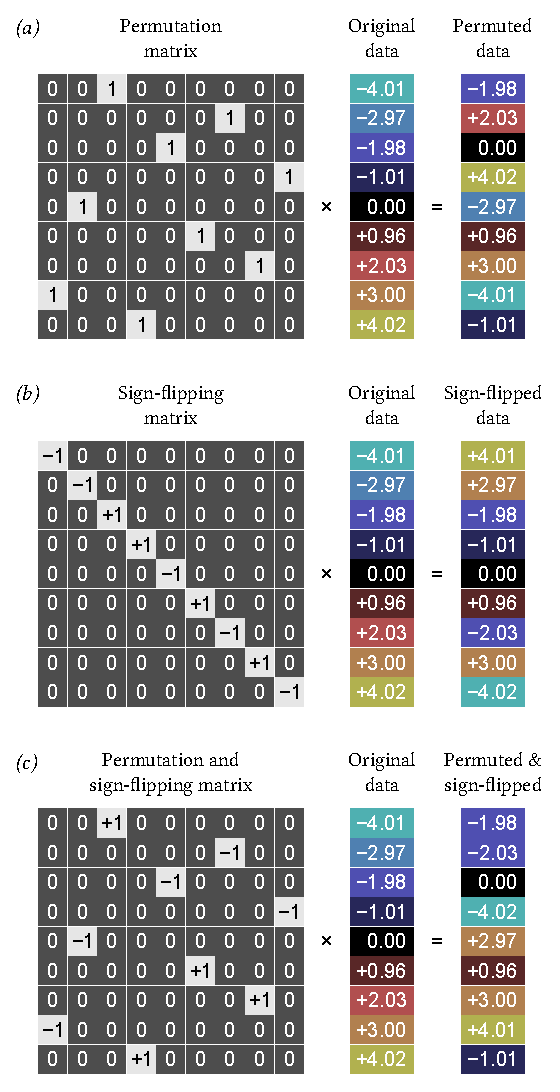
\includegraphics{images/pmatrices.eps}
\caption[Examples of permutation and sign-flipping matrices]{Examples of a permutation matrix \emph{(a)}, of a sign-flipping matrix \emph{(b)}, and of a matrix that does permutation and sign-flipping \emph{(c)}. Pre-multiplication by a permutation matrix shuffles the order of the data, whereas by a sign-flipping matrix changes the sign of each datapoint.}
\label{fig:pmatrices}
\end{figure}

Let $\boldsymbol{\hat{\beta}}_{\pi}$ and $T_{\pi}$ be, respectively, the estimated regression coefficients and the computed statistic for the permutation $\mathbf{P}_{\pi}$ or sign-flipping $\mathbf{S}_{\pi}$ drawn respectively from $\mathcal{P}$ or $\mathcal{S}$. The procedures to obtain a significance level with permutation tests consist of permuting or sign-flipping either the data, the model, or parts of the model, using $\mathbf{P}_{\pi}$ or $\mathbf{S}_{\pi}$, and constructing the empirical cdf of $T$, i.e., constructing $\mathsf{F}$, from which significance levels and confidence intervals can be obtained. Note that, as opposed to the parametric tests, $\mathsf{F}$ is not assumed to depend on any parameter.

The sole requirement for using permutation methods is that data are \emph{exchangeable}. That is, for a given set of variables, their joint probablility distribution does not change if the observations are permuted \citep{Good2002}. The exchangeability may be expressed in terms of exchangeable errors or of independent and symmetric errors, each of these weakening different assumptions of parametric methods.

\emph{Exchangeable errors} (\textsc{ee}) is the traditional permutation requirement. The formal statement is that, for any permutation $\mathbf{P}_{\pi} \in \mathcal{P}$, $\boldsymbol{\epsilon} \stackrel{\mathsf{d}}{=} \mathbf{P}_{\pi}\boldsymbol{\epsilon}$, where the symbol $\stackrel{\mathsf{d}}{=}$ denotes equality of distributions. In other words, the errors are considered exchangeable if their joint distribution is invariant with respect to permutation. Relative to the common parametric assumptions of independent, normally and identically distributed (iid) errors, the \textsc{ee} relaxes two aspects. First, normality is no longer assumed, although identical distributions are required. Second, the independence assumption is weakened slightly to allow exchangeability when the observations are not independent, but their joint distribution is maintained after permutation.\footnote{While exchangeability is a general condition that applies to any distribution, it might be useful to note that multivariate normal distribution is indeed exchangeable if the marginal distributions are uncorrelated, or when the off-diagonal elements of the variance-covariance matrix are equal \citep{Commenges2003}.}

\emph{Independent and symmetric errors} (\textsc{ise}) can be considered for measurements that arise, for instance, from differences between two groups, where the variances are not assumed to be the same \citep{Pesarin1995}. The formal statement for permutation under \textsc{ise} is that for any sign-flipping matrix $\mathbf{S}_{\pi} \in \mathcal{S}$, $\boldsymbol{\epsilon} \stackrel{\mathsf{d}}{=} \mathbf{S}_{\pi}\boldsymbol{\epsilon}$, that is, the joint distribution of the error terms is invariant with respect to sign-flipping. Relative to the parametric assumptions of independent, normally and identically distributed errors, this relaxes different aspects. First, normality is no longer assumed, although symmetry of distributions is required. Second, identical distributions for the error terms are no longer required, as each observation may have different variance, with symmetric shape. Independence is still required to allow sign-flipping of one observation without perturbing others.

If both \textsc{ee} and \textsc{ise} are plausible and available for a given model, the choice needs to consider the benefits and limitations of each. Although the \textsc{ee} does not require symmetry for the distribution of the error terms, it requires that the variances of the error terms are all equal (homoscedasticity), or have a structure that is compatible with the definition of blocks (discussed below). The \textsc{ise}, on the other hand, does not have this requirement, but can only be applied when the errors are symmetric.

There is yet another important aspect with respect to exchangeability. The experimental design may dictate \emph{blocks} of observations that are jointly exchangeable, allowing data to be permuted within block or, alternatively, that the blocks may themselves be exchangeable as a whole. This is the case, for instance, for designs that involve multiple observations from each subject. While permutation methods generally do not easily deal with correlated data, this special case of structured dependence can be easily accommodated. A summary of these properties is shown in Table~\ref{tab:assumptions}.

\begin{table}[!p]
\caption{Compared with parametric, permutation methods relax a number of assumptions and can be used in a wider variety of situations.}
\begin{center}
{\small
\begin{tabular}{@{}l@{}m{17mm}<{\centering}m{13mm}<{\centering}m{17mm}<{\centering}@{}}
\toprule
Assumptions                                & \textsc{ee} & \textsc{ise} & Parametric\\
\midrule
\multicolumn{4}{l}{\emph{With respect to the dependence structure between error terms:}}\\
Independent                                & {\color{blue}\ding{'63}}  & {\color{blue}\ding{'63}}  & {\color{blue}\ding{'63}}\\
Non-independent, well-structured blocks         & {\color{blue}\ding{'63}}  & {\color{blue}\ding{'63}}  & {\color{red}\ding{'67}}\\
Non-independent, exchangeable              & {\color{blue}\ding{'63}}  & {\color{red}\ding{'67}}   & {\color{red}\ding{'67}}\\
Non-independent, non-exchangeable          & {\color{red}\ding{'67}}   & {\color{red}\ding{'67}}   & {\color{red}\ding{'67}}\\
\midrule
\multicolumn{4}{l}{\emph{With respect to the distributions of the error terms:}}\\
Normal, identical                          & {\color{blue}\ding{'63}}  & {\color{blue}\ding{'63}}  & {\color{blue}\ding{'63}}\\
Symmetrical, identical                     & {\color{blue}\ding{'63}}  & {\color{blue}\ding{'63}}  & {\color{red}\ding{'67}}\\
Symmetrical, non-identical                 & {\color{red}\ding{'67}}   & {\color{blue}\ding{'63}}  & {\color{red}\ding{'67}}\\
Skewed, identical                          & {\color{blue}\ding{'63}}  & {\color{red}\ding{'67}}   & {\color{red}\ding{'67}}\\
Skewed, non-identical                      & {\color{red}\ding{'67}}   & {\color{red}\ding{'67}}   & {\color{red}\ding{'67}}\\
\bottomrule
\end{tabular}}
{\footnotesize
\begin{enumerate}
\item[{\color{blue}\ding{'63}}] Can be used directly if the assumptions regarding dependence structure and \newline distribution of the error terms are both met.\vspace{-2mm}
\item[{\color{red}\ding{'67}}] Cannot be used directly, or can be used in particular cases.
\end{enumerate}}
\end{center}
\label{tab:assumptions}
\end{table}


\subsubsection{Unrestricted exchangeability}
\label{sec:unrestricted}

If exchangeability is met for the whole set of observations, and in the absence of nuisance variables, a permutation test can be constructed by freely permuting the elements of $\mathbf{Y}$ or the rows of  $\mathbf{X}$. Permutation or sign-flipping matrices as shown in Figure~\ref{fig:pmatrices} can be used when appropriate and examples are given in \citet{Nichols2002}. However, in the presence of nuisance variables, the problem is more complex, and a number of approaches have been proposed \citep{Draper1966, Beaton1978, Still1981, Brown1982, Levin1983, Freedman1983, Oja1987, Gail1988, Welch1990, TerBraak1992, Kennedy1995, Edgington1995, Manly1997, Huh2001, Jung2006, Kherad2010}. Examples for some of these methods are given in Table~\ref{tab:methods}, and their performance were discussed comparatively by different authors \citep{Kennedy1995, Kennedy1996, Gonzalez1998, Anderson1999, Anderson2001, Anderson2003, OGorman2005, Dekker2007, Nichols2008, Ridgway2009}. Here we present and discuss the Freedman--Lane and the ter Braak methods, which, as we show in Section~\ref{sec:comparison}, produce the best results in terms of accuracy and power, a finding consonant with other studies \citep{Anderson1999, Dekker2007}.

\begin{table}[p]
\caption{A number of methods are available to obtain parameter estimates and construct a reference distribution in the presence of nuisance variables.}
\begin{center}
{\small
\begin{tabular}{@{}m{3.9cm}r@{\hspace{1.8mm}}c@{\hspace{2.2mm}}l}
\toprule
Method &
\multicolumn{3}{c}{Model\hspace*{18mm}}\\
\midrule
Exact$^{(a)}$ &
$\mathbf{Y} - \mathbf{Z}\boldsymbol{\gamma}$ &$=$& $\mathbf{P}_{\pi}\mathbf{X}\boldsymbol{\beta} + \boldsymbol{\epsilon}$ \\
Draper--Stoneman$^{(b)}$ & 
$\mathbf{Y}$ &$=$& $\mathbf{P}_{\pi}\mathbf{X}\boldsymbol{\beta} + \mathbf{Z}\boldsymbol{\gamma} + \boldsymbol{\epsilon}$ \\
Still--White$^{(c)}$ &
$\mathbf{P}_{\pi}\mathbf{R}_{\mathbf{Z}}\mathbf{Y}$ &$=$& $\mathbf{X}\boldsymbol{\beta} + \boldsymbol{\epsilon}$  \\
Freedman--Lane$^{(d)}$ &
$\left(\mathbf{P}'_{\pi}\mathbf{R}_{\mathbf{Z}}+\mathbf{H}_{\mathbf{Z}}\right)\mathbf{Y}$ &$=$& $\mathbf{X}\boldsymbol{\beta} + \mathbf{Z}\boldsymbol{\gamma}+\boldsymbol{\epsilon}$ \\
ter Braak$^{(e)}$ &
$\left(\mathbf{P}'_{\pi}\mathbf{R}_{\mathbf{M}}+\mathbf{H}_{\mathbf{M}}\right)\mathbf{Y}$ &$=$& $\mathbf{X}\boldsymbol{\beta} + \mathbf{Z}\boldsymbol{\gamma}+\boldsymbol{\epsilon}$ \\
Kennedy$^{(f)}$ &
$\mathbf{P}'_{\pi}\mathbf{R}_{\mathbf{Z}}\mathbf{Y}$ &$=$& $\mathbf{R}_{\mathbf{Z}}\mathbf{X}\boldsymbol{\beta} +  \boldsymbol{\epsilon}$ \\
Manly$^{(g)}$ &
$\mathbf{P}'_{\pi}\mathbf{Y}$ &$=$& $\mathbf{X}\boldsymbol{\beta} + \mathbf{Z}\boldsymbol{\gamma} + \boldsymbol{\epsilon}$\\
Huh--Jhun$^{(h)}$ &
$\mathbf{P}'_{\pi}\mathbf{Q}'\mathbf{R}_{\mathbf{Z}}\mathbf{Y}$ &$=$& $\mathbf{Q}'\mathbf{R}_{\mathbf{Z}}\mathbf{X}\boldsymbol{\beta} +  \boldsymbol{\epsilon}$\\
Smith$^{(i)}$ &
$\mathbf{Y}$ &$=$& $\mathbf{P}_{\pi}\mathbf{R}_{\mathbf{Z}}\mathbf{X}\boldsymbol{\beta} + \mathbf{Z}\boldsymbol{\gamma} + \boldsymbol{\epsilon}$ \\
Parametric$^{(j)}$ &
$\mathbf{Y}$ &$=$& $\mathbf{X}\boldsymbol{\beta} + \mathbf{Z}\boldsymbol{\gamma} + \boldsymbol{\epsilon},\;\; \boldsymbol{\epsilon}\sim\mathcal{N}(\mu,\sigma^2\mathbf{I})$ \\
\bottomrule
\end{tabular}}
\end{center}
{\footnotesize
$(a)$ In the Exact method, the true $\boldsymbol{\gamma}$ is known and does not need to be estimated. Since it is known, $\mathbf{Z}\boldsymbol{\gamma}$ can be subtracted from $\mathbf{Y}$, and only $\boldsymbol{\beta}$ needs to be estimated. Permutation can be performed as for simple regression. The Exact method is used for comparison with the others in the simulations presented in Section~\ref{sec:comparison}.
$(b)$ \citet{Draper1966}. This method was called ``Shuffle~Z'' by \citet{Kennedy1995}, and using the same notation adopted here, it would be called ``Shuffle~$\mathbf{X}$''.
$(c)$ \citet{Still1981, Levin1983, Gail1988}.
$(d)$ \citet{Freedman1983}.
$(e)$ \citet{TerBraak1992}. The null distribution for this method considers $\boldsymbol{\hat{\beta}}_{\pi} = \boldsymbol{\hat{\beta}}$, i.e., the permutation happens under the alternative hypothesis, rather than the null.
$(f)$ \citet{Kennedy1995, Kennedy1996}. This method was referred to as ``Residualize both Y and Z'' in the original publication, and using the same notation adopted here, it would be called ``Residualize both Y and X''. When $\mathbf{X}$ and $\mathbf{Z}$ are orthogonal, this method is equivalent to Still--White.
$(g)$ \citet{Manly1997}.
$(h)$ \citet{Huh2001, Jung2006, Kherad2010}. $\mathbf{Q}$ is a $n \times n'$ matrix, where $n'=n-q$ is the rank of $\mathbf{R}_{\mathbf{Z}}$. $\mathbf{Q}$ is computed through Schur decomposition of $\mathbf{R}_{\mathbf{Z}}$, such that $\mathbf{R}_{\mathbf{Z}}=\mathbf{Q}\mathbf{Q}'$ and $\mathbf{I}_{n' \times n'}=\mathbf{Q}'\mathbf{Q}$. For this method, $\mathbf{P}_{\pi}$ is $n' \times n'$.
$(i)$ The Smith method was suggested by a referee of \citet{OGorman2005}, and later presented by \citet{Nichols2008} and discussed by \citet{Ridgway2009}.
$(j)$ The parametric method does not use permutations, being instead based on distributional assumptions.\
$\square$ For all the methods, the left side of the equations contains the regressand, the right side the regressors and error terms. The unpermuted models can be obtained by replacing $\mathbf{P}_{\pi}$ for $\mathbf{I}$. Even for the unpermuted models, and even if $\mathbf{X}$ and $\mathbf{Z}$ are orthogonal, not all these methods produce the same error terms $\boldsymbol{\epsilon}$. This is the case for the Kennedy, Huh--Jhun and Smith methods. If the permutations are constructed obeying certain rules (e.g.\ lexicographic or respecting blocks), permuting with $\mathbf{P}_{\pi}$ will not produce the same results as permuting with $\mathbf{P}'_{\pi}$, and correct matrix transposition has to be observed to construct the correct empirical distribution.}
\label{tab:methods}
\end{table}

The \emph{Freedman--Lane procedure} \citep{Freedman1983} can be performed through the following steps:

\begin{enumerate}
\item Regress $\mathbf{Y}$ against the full model that contains both the effects of interest and the nuisance variables, i.e.\ $\mathbf{Y} = \mathbf{X}\boldsymbol{\beta} + \mathbf{Z}\boldsymbol{\gamma} + \boldsymbol{\epsilon}$. Use the estimated parameters $\boldsymbol{\hat{\beta}}$ to compute the statistic of interest, and call this statistic $T$.
\item Regress $\mathbf{Y}$ against a reduced model that contains only the nuisance effects, i.e.\ $\mathbf{Y} = \mathbf{Z}\boldsymbol{\gamma} + \boldsymbol{\epsilon}_{\mathbf{Z}}$, obtaining estimated parameters $\boldsymbol{\hat{\gamma}}$ and estimated residuals $\boldsymbol{\hat{\epsilon}}_{\mathbf{Z}}$.
\item Compute a set of permuted data $\mathbf{\tilde{Y}}_{\pi}$. This is done by pre-multiplying the residuals from the reduced model produced in the previous step, $\boldsymbol{\hat{\epsilon}}_{\mathbf{Z}}$, by a permutation matrix, $\mathbf{P}'_{\pi}$, then adding back the estimated nuisance effects, i.e.\ $\mathbf{\tilde{Y}}_{\pi} = \mathbf{P}'_{\pi}\boldsymbol{\hat{\epsilon}}_{\mathbf{Z}} + \mathbf{Z}\boldsymbol{\hat{\gamma}}$. 
\item Regress the permuted data $\mathbf{\tilde{Y}}_{\pi}$ against the full model, i.e.\ $\mathbf{\tilde{Y}}_{\pi} = \mathbf{X}\boldsymbol{\beta} + \mathbf{Z}\boldsymbol{\gamma} + \boldsymbol{\epsilon}$, and use the estimated $\boldsymbol{\hat{\beta}}_{\pi}$ to compute the statistic of interest. Call this statistic $T_{\pi}$.
\item Repeat the Steps 2--4 many times to build the reference distribution of $T_{\pi}$ under the null hypothesis.
\item Count how many times $T_{\pi}$ was found to be equal or larger than $T$, and divide by the number of permutations. The result is the $p$-value, the probability of obtaining a statistic larger than $T$ due to chance alone.
\end{enumerate}

For the Steps 2 and 3, it is not necessary to actually fit the reduced model at each point in the image. The permuted dataset can equivalently be obtained as $\mathbf{\tilde{Y}}_{\pi} = \left(\mathbf{P}'_{\pi}\mathbf{R}_{\mathbf{Z}}+\mathbf{H}_{\mathbf{Z}}\right)\mathbf{Y}$, which is particularly efficient for neuroimaging applications, as the term $\mathbf{P}'_{\pi}\mathbf{R}_{\mathbf{Z}}+\mathbf{H}_{\mathbf{Z}}$ is constant for all points and, therefore, needs to be computed just once. Another useful simplification can be done if $\mathbf{X}$ and $\mathbf{Z}$ are orthogonal. In this case, the regressors in $\mathbf{Z}$ have no overlap with those in $\mathbf{X}$, and so, add the nuisance variables back in Step 3, then regressing them out again in Step 4 is redundant. In this case, the model can be expressed simply as $\mathbf{P}'_{\pi}\mathbf{R}_{\mathbf{Z}}\mathbf{Y}=\mathbf{X}\boldsymbol{\beta}+\boldsymbol{\epsilon}$, implying that the permutations can actually be performed just by permuting the rows of the residual-forming matrix $\mathbf{R}_{\mathbf{Z}}$ and fitting a reduced model with just $\mathbf{X}\boldsymbol{\beta}$ or, equivalently, permuting\footnote{This simplification renders the Freedman--Lane equivalent to the Still--White method (Table~\ref{tab:methods}).} the rows of $\mathbf{X}$ in this same reduced, permuted model with only the covariates of interest, i.e., $\mathbf{R}_{\mathbf{Z}}\mathbf{Y}=\mathbf{P}_{\pi}\mathbf{X}\boldsymbol{\beta}+\boldsymbol{\epsilon}$. If $\mathbf{M}$ is partitioned using the methods discussed in Section~\ref{sec:partitioning}, the columns of $\mathbf{X}$ and $\mathbf{Z}$ are indeed orthogonal.

The rationale for this permutation method is that, if the null hypothesis is true, then $\boldsymbol{\beta}=\mathbf{0}$, and so the residuals from the reduced model with only nuisance variables, $\boldsymbol{\epsilon}_{\mathbf{Z}}$, should not be different than the residuals from the full model, $\boldsymbol{\epsilon}$, and can, therefore, be used to create the reference distribution from which $p$-values can be obtained.

The \emph{ter Braak procedure} \citep{TerBraak1992} differs from the Freedman--Lane method in that the residuals from the full model are permuted, rather than the residuals from the reduced model. The method can be performed through the following steps:

\begin{enumerate}
\item Regress $\mathbf{Y}$ against the full model that contains both the effects of interest and the nuisance variables, i.e.\ $\mathbf{Y} = \mathbf{X}\boldsymbol{\beta} + \mathbf{Z}\boldsymbol{\gamma} + \boldsymbol{\epsilon}$. Use the estimated parameters $\boldsymbol{\hat{\beta}}$ to compute the statistic of interest for the hypothesis $\boldsymbol{\beta}=\boldsymbol{0}$, and call this statistic $T$.
\item Compute a set of permuted data $\mathbf{\tilde{Y}}_{\pi}$. This is done by pre-multiplying the residuals from the previous step, $\boldsymbol{\hat{\epsilon}}$, by a permutation matrix, $\mathbf{P}'_{\pi}$, then adding back all the estimated effects, i.e.\ $\mathbf{\tilde{Y}}_{\pi} = \mathbf{P}'_{\pi}\boldsymbol{\hat{\epsilon}} + \mathbf{X}\boldsymbol{\hat{\beta}} + \mathbf{Z}\boldsymbol{\hat{\gamma}}$.
\item Regress the permuted data $\mathbf{\tilde{Y}}_{\pi}$ against the full model, i.e.\ $\mathbf{\tilde{Y}}_{\pi} = \mathbf{X}\boldsymbol{\beta} + \mathbf{Z}\boldsymbol{\gamma} + \boldsymbol{\epsilon}$, and use the estimated $\boldsymbol{\hat{\beta}}_{\pi}$ to compute the statistic of interest for the hypothesis $\boldsymbol{\beta}=\boldsymbol{\hat{\beta}}$. Call this statistic $T_{\pi}$.
\item Repeat the Steps 2--3 many times to build the reference distribution of $T_{\pi}$ under the \emph{alternative} hypothesis.
\item Count how many times $T_{\pi}$ was found to be equal or larger than $T$, and divide by the number of permutations. The result is the $p$-value, the probability of obtaining a statistic larger than $T$ due to chance alone.
\end{enumerate}

As with the Freedman--Lane case, some simplifications apply. The permuted dataset can be obtained as $\mathbf{\tilde{Y}}_{\pi} = \left(\mathbf{P}'_{\pi}\mathbf{R}_{\mathbf{M}} + \mathbf{H}_{\mathbf{M}}\right)\mathbf{Y}$, with similar computational benefits for neuroimaging applications. Moreover, it is immaterial to add back the estimated effects in Step 2 and  compute a statistic for the alternative hypothesis, when the same distribution can be computed by fitting the model $\mathbf{P}'_{\pi}\boldsymbol{\hat{\epsilon}} = \mathbf{P}'_{\pi}\mathbf{R}_{\mathbf{M}}\mathbf{Y} = \mathbf{X}\boldsymbol{\beta} + \mathbf{Z}\boldsymbol{\gamma} + \boldsymbol{\tilde{\epsilon}}$ and computing the statistic $T_{\pi}$ for the null.

The rationale for this permutation method is that, by replacing the residuals from the restricted model by the residuals from the full model, a gain in power could be obtained, analogously as gains observed with a similar strategy for bootstrapping \citep{Hall1989}. In the ter Braak method, the reference distribution is computed under the alternative hypothesis. This is because the variability of the permuted, estimated values $\boldsymbol{\hat{\beta}}_{\pi}$ around the unpermuted estimate $\boldsymbol{\hat{\beta}}$ reproduces the variability of $\boldsymbol{\hat{\beta}}$ around the true, unknown parameter $\boldsymbol{\beta}$. In order to adequately capture this variability, a pivotal statistic is mandatory for $T$, in addition to all the reasons earlier in this article.

For both the Freedman--Lane and the ter Braak procedures, if the errors are independent and symmetric (\textsc{ise}), the permutation matrices $\mathbf{P}_{\pi}$ can be replaced for sign-flipping matrices $\mathbf{S}_{\pi}$.

\subsubsection{Restricted exchangeability}

Some experimental designs involve multiple observations from each subject, or the subjects may come from groups that may possess known characteristics that may render their distributions not perfectly comparable. Both situations violate the exchangeability principle. However, when the dependence between observations has a block structure, this structure can be taken into account when permuting the model, restricting the set of all otherwise possible permutations to only those that respect the relationship between observations \citep{Pesarin2001}. We call the blocks of related observations as \emph{dependent data blocks} (\textsc{ddb}). The \textsc{ee} and \textsc{ise} assumptions are then asserted at the block level, rather than for each observation individually. The experimental hypothesis and the study design determine how the \textsc{ddb} should be formed and how the permutation or sign-flipping matrices should be constructed. The Freedman--Lane and the ter Braak procedures can be applied similarly as above.

\paragraph{Within-block exchangeability}

Blocks of observations that share the same dependence, either assumed or known in advance, can be defined such that \textsc{ee} are asserted with respect to these blocks only, and the empirical distribution is constructed by permuting exclusively within block, as shown in Figure~\ref{fig:within-block}. Once the blocks have been defined, the regression of nuisance variables and the construction of the reference distribution follow the Freedman--Lane or ter Braak strategies, as above. The \textsc{ise}, when applicable, is transparent to this kind of block structure, so that the sign flips occur as under unrestricted exchangeability. Yet, if the variances are not only known to differ, but also their (relative) magnitudes are known exactly, the analysis can proceed using weighted least squares (\textsc{wls)}, using for weighting either the (known) inverted covariance matrix of the residuals, or of the actual observations. The second case may be appropriate when, for instance, some of the observations were obtained by a different measuring device or observer, either of which being known to produce measurements with different variability. In any of these cases, the covariance matrix must be diagonal. With \textsc{wls}, the \textsc{ddb} structure for within-block exchangeability can be ignored, and permutations or sign flips can be done without the constraints imposed by the blocks.\footnote{An example use of \textsc{wls} and permutation, using the Draper--Stoneman method, is given in \citet{OGorman2005}.}

\begin{figure}[!p]
\centering
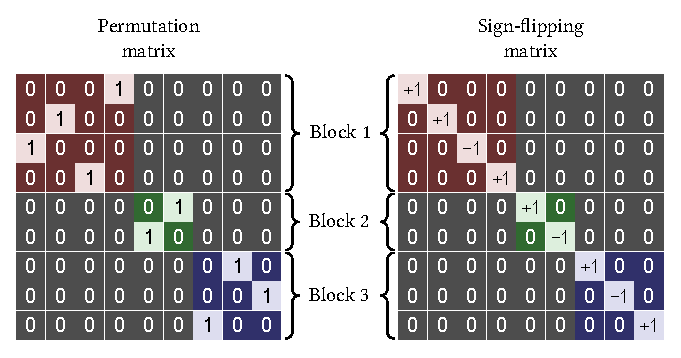
\includegraphics{images/within-block.eps}
\caption[Example of a within-block permutation matrix.]{\emph{Left:} Example of a permutation matrix that shuffles data within block only. The blocks are not required to be of the same size. The elements outside the diagonal blocks are always equal to zero, such that data cannot be swapped across blocks. \emph{Right:} Example of a sign-flipping matrix. Differently than within-block permutation matrices, here sign-flipping matrices are transparent to the definitions of the blocks, such that the blocks do not need to be taken into account.}
\label{fig:within-block}
\end{figure}

\paragraph{Whole-block exchangeability}

When multiple measurements per subject are analysed, unrestricted exchangeability cannot, again, be assumed. Instead, blocks can be constructed such that they include all observations collected per subject. Differently than in within-block exchangeability, here each block of residuals is permuted as a whole for \textsc{ee} and, consequently, all blocks must be of the same size, i.e., each must contain the same number of observations. For \textsc{ise}, when applicable, the signs of the residuals are flipped for each block as a whole and, as a consequence, the blocks do not have to be all of the same size. Examples of permutation and sign-flipping matrices for whole block permutation are shown in Figure~\ref{fig:whole-block}.

\begin{figure}[!p]
\centering
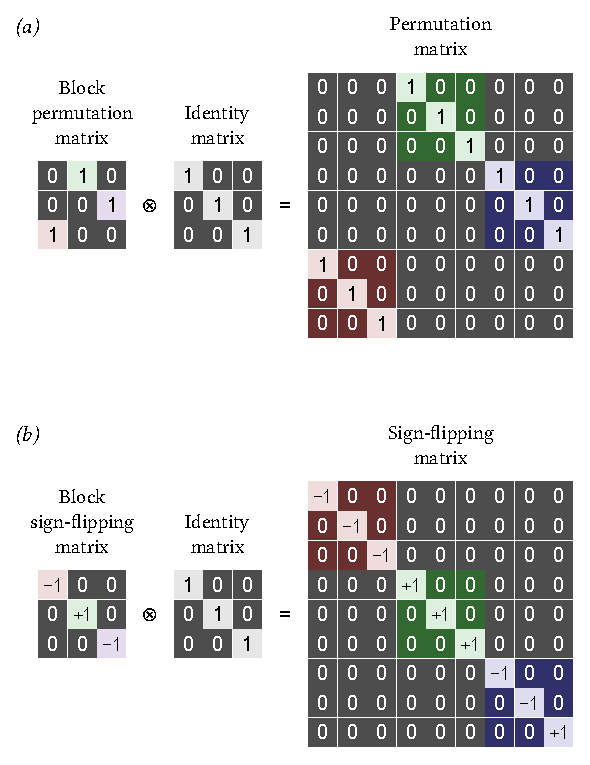
\includegraphics{images/whole-block.eps}
\caption[Example of whole-block permutation and sign-flipping matrices.]{\emph{(a)} Example of a permutation matrix that shuffles whole blocks of data. The blocks need to be of the same size. \emph{(b)} Example of a sign-flipping matrix that changes the signs of the blocks as a whole. Both matrices can be constructed by the Kronecker product (represented by the symbol $\otimes$) of a permutation or a sign-flipping matrix, either with size determined by the number of blocks, by an identity matrix with size determined by the number of observations per block.}
\label{fig:whole-block}
\end{figure}

\subsection{Number of permutations} 

For a study with $n$ observations, the maximum number possible permutations, $\pi^{\mathcal{P}}_{\text{max}}$, is simply $n!$, and the maximum number of possible sign flips is $2^n$. However, in the presence of $B$ dependent data blocks that are exchangeable as a whole, the maximum number of possible permutations drops to no more than $B!$, and the maximum number of sign flips to $2^B$. For designs where data is only exchangeable within-block, the maximum number of possible permutations is $\prod_{b=1}^{B} n_{b}!$, where $n_{b}$ is the number of observations for the $b$-th block, and the maximum number of sign flips continues to be $2^n$. However, the actual number of possible permutations may be smaller depending on the null hypothesis, the permutation strategy, or other aspects of the study design. If there are discrete covariates (categorical), or if there are ties among continuous regressors, many permutations may not alter the model at all, and so, are redundant (synonymous). The maximum number of permutations can be calculated generically from the design matrix observing the number of repeated rows in $\mathbf{X}$ for the Freedman--Lane method, or in $\mathbf{M}$ for the ter Braak method. The maximum number of possible permutations or sign flips, for different restrictions on exchangeability, is shown in Table~\ref{tab:numperm}.

\begin{table}[p]
\caption{Maximum number of unique permutations, $\pi^{\mathcal{P}}_{\text{max}}$, considering exchangeability blocks.}
\begin{center}
{\small
\begin{tabular}{@{}m{62mm}<{\raggedright}m{44mm}<{\centering}@{}m{15mm}<{\centering}@{}}
\toprule
Exchangeability & \textsc{ee}   & \textsc{ise}\\
\midrule
Unrestricted & \[n!\] & \[2^n\]\\
\midrule
Unrestricted, repeated rows & \[n!\prod_{m=1}^M \frac{1}{n_m!}\] & \[2^n\] \\
\midrule
Within-block & \[\prod_{b=1}^{B} n_{b}!\] & \[2^n\] \\
\midrule
Within-block, repeated rows & \[\prod_{b=1}^{B} n_{b}! \prod_{m=1}^{M|b} \frac{1}{n_{m|b}!}\] & \[2^n\] \\
\midrule
Whole-block  & \[B!\] & \[2^B\]\\
\midrule
Whole-block, repeated blocks  & \[B!\prod_{\tilde{m}=1}^{\tilde{M}} \frac{1}{n_{\tilde{m}}!}\] & \[2^B\]\\
\bottomrule
\end{tabular}}
\end{center}
{\footnotesize
$B$ is the number of dependent data blocks (\textsc{ddb}),
$M$ is the number of distinct rows in $\mathbf{X}$,
$M|b$ is the number of distinct rows in $\mathbf{X}$ within the $b$-th block,
$\tilde{M}$ is the number of distinct blocks of rows in $\mathbf{X}$,
$n$ is the number of observations,
$n_b$ is the number of observations in the $b$-th block,
$n_m$ is the number of times each of the $M$ distinct rows occurs in $\mathbf{X}$,
$n_{m|b}$ is the number of times each of the $m$-th unique row occurs within the $b$-th block, and
$n_{\tilde{m}}$ is the number of times each of the $\tilde{M}$ distinct blocks occurs in $\mathbf{X}$.}
\label{tab:numperm}
\end{table}

Even considering the restrictions dictacted by the study design, the number of possible permutations tends to be very large, even for samples of moderate size, and grows very rapidly as subjects are added. When the number of possible permutations is extremely large, not all the possible permutations need to be performed for the test to be valid \citep{Dwass1957, Chung1958}, and the resulting procedure will be almost exact \citep{Edgington1969}. Only a subset of $\mathcal{P}$ or $\mathcal{S}$ needs to be used, and the number can be chosen according to the availability of computational resources and considerations about power. The smallest $p$-value that can be obtained is given by $1/\pi_{\text{\#}}$, where $\pi_{\text{\#}}$ is the number of permutations performed, including the unpermuted model, and often much smaller than the maximum number of possible permutations.

To efficiently avoid permutations that do not change the design matrix, the Algorithm ``\textsc{l}'' \citep{Knuth2005} can be used. This algorithm is simple and generates only permutations that are unique, i.e., in the presence of repeated elements, it avoids synonymous permutations. This is appropriate when enumerating all possible permutations. However, the algorithm produces sequentially permutations that are in lexicographic order. Although this can be advantageous in other settings, here this behaviour can be problematic when running only a subset of $\mathcal{P}$, and has potential to bias the results. For imaging applications, it is in general computationally less expensive to shuffle many times a sequence of values and store these permuted sequences, than actually fit the permuted model for all image points. As a consequence, the problem with lexicographically ordered permutations can be solved by generating all the possible permutation and/or sign-flipping matrices, and randomly drawing $\pi_{\text{\#}}$ elements from $\mathcal{P}$ to do the actual shuffling of the model. If, however, $\pi^{\mathcal{P}}_{\text{max}}$ is huge, a few orders of magnitude larger than $\pi_{\text{\#}}$, the procedure can be conducted without attention to repeated permutations using simple shuffling of the data. This strategy is known as \emph{conditional Monte Carlo} (\textsc{cmc}) \citep{Trotter1956, Pesarin2010}, as each of the random realisations is conditional on the available observed data.\footnote{In fact, as long as $\mathcal{P}$ is sampled uniformly, repeated permutations are not an issue unless for very small samples, in which case exact p-values can only be observed asymptotically.}

Sign-flipping matrices, on the other hand, can be listed using a numeral system with radix 2, and the sign-flipped models can be performed without appealing to \textsc{cmc}, even if $\pi^{\mathcal{P}}_{\text{max}}$ is huge. The simplest strategy is to use the binary numeral system that uses the digits $0$ and~$1$, treating the digit 0 as $-1$ when assembling the matrix. In a binary system, each sign-flipping matrix is also its own numerical identifier, such that avoiding repeated sign-flippings is trivial. The binary representation can be converted to and from radix 10 if needed, e.g., to allow easier human readability.

For within-block exchangeability, permutation matrices are constructed within-block, then concatenated along their diagonal to assemble $\mathbf{P}_{\pi}$, which also has a block structure. The elements outside the blocks are filled with zeros as needed  (Figure~\ref{fig:within-block}). The block definitions can be ignored for sign-flipping matrices for designs where \textsc{ise} is asserted within-block. For whole-block exchangeability, permutation and sign-flipping matrices are generated by treating each block as an element, and the final $\mathbf{P}_{\pi}$ or $\mathbf{S}_{\pi}$ are assembled via Kronecker multiplication by an identity matrix of the same size as the blocks (Figure~\ref{fig:whole-block}).

The considerations above refer to the number of possible permutations for a given design matrix, and can be computed once $\mathbf{M}$ has been designed and partitioned according to the constrast into $\mathbf{X}$ and $\mathbf{Z}$. However, for many study designs that use categorical variables (i.e.\ ``factors'' with a discrete number of ``levels''), $\pi^{\mathcal{P}}_{\text{max}}$ or $\pi^{\mathcal{S}}_{\text{max}}$ can be computed before the design matrix is assembled. Table~\ref{tab:taxonomy} shows a list of common study designs, and the number of possible permutations when the errors can be considered exchangeable or independent and symmetric.

\begin{table}[p]
\caption{Maximum number of unique permutations, $\pi^{\mathcal{P}}_{\text{max}}$, for some common designs.}
\begin{center}
{\small
\begin{tabular}{@{}l@{}m{57mm}<{\centering}@{}m{10mm}<{\centering}@{}}
\toprule
Model name & \textsc{ee} & \textsc{ise}\\
\midrule
One sample $t$-test & \vspace*{3mm}--\vspace*{3mm} & $2^{n}$ \\
\midrule
Two-sample $t$-test & \vspace*{3mm}$\dbinom{n}{n_1}$ or $\dbinom{n}{n_2}$\vspace*{3mm} & $2^{n}$ \\
\midrule
Paired $t$-test & \vspace*{3mm}$2^{B}$\vspace*{3mm} & $2^{B}$ \\
\midrule
Tripled $t$-test$^{(a)}$ & \vspace*{3mm}$(3!)^{B}$\vspace*{3mm}  & $2^{B}$ \\
\midrule
One-way repeated-measures \textsc{anova}$^{(b)}$ & \vspace*{3mm}$K!$\vspace*{3mm} & $2^{B}$ \\
\midrule
Two-way repeated-measures \textsc{anova}$^{(c)}$ & \vspace*{3mm}$K!J!$\vspace*{3mm} & $2^{B}$ \\
\midrule
Two-way repeated-measures \textsc{anova}$^{(d)}$ & \vspace*{3mm}$J!$\vspace*{3mm} & $2^{B}$ \\
\midrule
One-way between-subjects \textsc{anova}$^{(e)}$  & \vspace*{3mm}$\dbinom{n}{n_1,n_2,\ldots,n_K}$\vspace*{3mm} & $2^{n}$\\
\midrule
Two-way between-subjects \textsc{anova}$^{(f)}$  & \vspace*{3mm}$\dbinom{n}{n_1,\ldots,n_K}$ or $\dbinom{n}{n_1,\ldots,n_J}$\vspace*{3mm} & $2^{n}$ \\
\bottomrule
\end{tabular}}
\end{center}
{\footnotesize
($a$) \textsc{ee} can be used if data is exchangeable within-subject.
($b$) $K$ images per subject, one for each of factor level. \textsc{ee} can be used if data is exchangeable within-subject.
($c$) Two factors, both within subject, and $K \times J$ images per subject, one for each possible combination of levels of the two intrasbuject factors. \textsc{ee} can be used if data is exchangeable within-subject.
($d$) Two factors, one within subject, one between subjects. $K$ images per subject, one for each intrasbuject factor level. Subjects assigned to exactly one of $J$ factor levels.
($e$) One image per subject, each subject assigned to one of $K$-levels of a factor.
($f$) One image per subject, each subject assigned to a pair of factor levels, one of $K \times J$ possible, where there is one $K$-level factor and one $J$-level factor.}
\label{tab:taxonomy}
\end{table}

\subsection{Multiple testing}

Differently than with parametric methods, correction for multiple testing using permutation methods does not require the introducion of more assumptions. For familywise error rate correction (\textsc{fwer}), the method was described by \citet{Nichols2002}. As the statistics $T_{\pi}$ are calculated for each permutation $\pi$ to build the reference distribution at each point, the maximum value of $T_{\pi}$ across the image, $T_{\pi}^{\text{max}}$, is also recorded for each permutation, and its empirical distribution is obtained. For each test in the image, an \textsc{fwer}-corrected $p$-value can then be obtained by computing the proportion of $T_{\pi}^{\text{max}}$ that is above $T$ for each test. A single \textsc{fwer} threshold can also be applied to the statistical map of $T$ values using the distribution of $T_{\pi}^{\text{max}}$. The same strategy is used for statistics that combine spatial extent of signals, such as cluster size, cluster mass, and \textsc{tfce}.

The $p$-values under the null hypothesis are uniformly distributed in the interval $[0,1]$. As a consequence, the $p$-values are too pivotal quantities, and can be used for multiple-testing in a similar fashion as above. In this case, the minimum $p$-value, $p_{\pi}^{\text{min}}$, instead of $T_{\pi}^{\text{max}}$ is used \citep{Pantazis2005}. Correction based on false-discovery rate (\textsc{fdr}) can also be used once the uncorrected $p$-values have been obtained for each point in the image. Either a single \textsc{fdr} threshold can be applied to the map of uncorrected $p$-values \citep{Benjamini1995, Genovese2002} or, alternatively, an \textsc{fdr}-adjusted $p$-value can be calculated at each point of the image \citep{Yekutieli1999}.

\subsection{The \texttt{randomise} algorithm}

A generic algorithm for permutation inference on contrasts of the \textsc{glm} parameter estimates using the Freedman--Lane method is presented (Algorithm~1). Modifications for the ter Braak method are trivial and may include, for instance, the simplification to estimate the residuals just once for all contrasts. For this algorithm, consider $\mathbf{Y}$ as a four-dimensional array, being the first three for the dimensions in space, and the last for an observation index. A variable $\mathbf{v}=[x, y, z]$ is used to specify the point position is space, so that the vector of $n$ different observations per point is represented as $\mathbf{Y}[\mathbf{v}]$. A set $\mathcal{C}$ of contrasts is specified, as well as the unpartitioned design matrix $\mathbf{M}$. Indicator variables are used to specify whether the errors should be treated as exchangeable ($\textsc{ee}=\textsc{true}$), independent and symmetric ($\textsc{ise}=\textsc{true}$), or both, which allows for permutations to happen together with sign-flipping. A positive integer is specified as the maximum number permutations to be performed, $\pi_{\text{\#}}$. Optionally, a $n \times 1$ vector $\mathbf{b}$ is provided to indicate the $B$ dependent data blocks that group the observations, along with an indicator variable $\textsc{pb}$ that informs whether blocks should be permuted as a whole ($\textsc{pb} = \textsc{true}$), or if permutations should happen within block only ($\textsc{pb} = \textsc{false}$). Also optionally, a variable $\mathbf{W}$, of the same size as $\mathbf{Y}$, is used for weighting in a \textsc{wls} regression. The fourth dimension of $\mathbf{W}$ contains the diagonal elements of the covariance matrix between the observations at each voxel. As the off-diagonal elements are all zero, the matrix can be represented as a single vector per voxel with no loss of information.

\vspace{8mm}
\singlespacing
% \hrule
% \vspace{2.5mm}
\noindent \textsf{Algorithm 1: The \texttt{randomise} algorithm.}\\
\HRule
\vspace{2mm}
{\small
\begin{algorithmic}[1]
\Require $\mathbf{Y}, \mathbf{M}, \mathcal{C}, \textsc{ee}, \textsc{ise}, \pi_{\text{\#}}$. \textbf{Optional:} $\mathbf{b}, \textsc{pb}, \mathbf{W}$.
\Comment{Input variables.}
\If{\textlnot\ \textsf{exist}($\mathbf{b}$)}
\Comment{If $\mathbf{b}$ was not provided.}
\State $\mathbf{b} \leftarrow \mathbf{1}_{n \times 1}$
\Comment{A vector of ones is used for $\mathbf{b}$.}
\State $\textsc{pb} \leftarrow \textsc{false}$
\Comment{Permutations happen within the single block.}
\EndIf
\If{\textsf{exist}($\mathbf{W}$)}
\Comment{If $\mathbf{W}$ was provided.}
\ForAll{$\mathbf{v}$}
\Comment{For each image point.}
\State $\mathbf{Y}[\mathbf{v}] \leftarrow \mathbf{Y}[\mathbf{v}] \oslash \mathbf{W}[\mathbf{v}]$
\Comment{Weight data. Elementwise division along $n$.}
\ForAll{$c$}
\Comment{For each column $\mathbf{m}_c$ of $\mathbf{M}$.}
\State $\mathbf{m}_c[\mathbf{v}] \leftarrow \mathbf{m}_c[\mathbf{v}] \oslash \mathbf{W}[\mathbf{v}]$
\Comment{Weight the model, for each point.}
\EndFor
\EndFor
\EndIf
\ForAll{$\mathbf{C} \in \mathcal{C}$}
\Comment{For each contrast.}
\State $\mathbf{X}, \mathbf{Z} \leftarrow \text{\textsf{partition}}(\mathbf{M}, \mathbf{C})$
\Comment{Partition the model.}
\State $\pi^{\mathcal{P}}_{\text{max}}, \pi^{\mathcal{S}}_{\text{max}} \leftarrow \text{\textsf{calc\_maxperm}}(\mathbf{X}, \mathbf{b}, \textsc{pb}, \textsc{ee}, \textsc{ise})$
\Comment{Max.\ possible shufflings.}
\If {$\textsc{ee}$}
\Comment{If errors are exchangeable.}
\If {$\pi_{\#} \geqslant \pi^{\mathcal{P}}_{\text{max}}$}
\Comment{Exhaustive or too many permutations requested.}
\State $\tilde{\mathcal{P}} \leftarrow \text{\textsf{algorithm\_L}}(\mathbf{X}, \mathbf{b}, \textsc{pb})$
\Comment{List all possible permutations.}
\Else
\State $\tilde{\mathcal{P}} \leftarrow \text{\textsf{shuffle\_randomly}}(\mathbf{X}, \mathbf{b}, \textsc{pb}, \pi_{\#})$
\Comment{Ignore possible repeated $\mathbf{P}_{\pi}$.}
\EndIf
\EndIf
\If {$\textsc{ise}$}
\Comment{If errors are independent and symmetric.}
\If {$\pi_{\#} \geqslant \pi^{\mathcal{S}}_{\text{max}}$}
\Comment{Exhaustive or too many sign-flips requested.}
\State $\tilde{\mathcal{S}} \leftarrow \text{\textsf{list\_signflips}}(n, \mathbf{b}, \textsc{pb})$
\Comment{List all possible sign-flippings.}
\Else
\State $\tilde{\mathcal{S}} \leftarrow \text{\textsf{signflip\_randomly}}(n, \mathbf{b}, \textsc{pb}, \pi_{\#})$
\Comment{Ignore possible repeated $\mathbf{S}_{\pi}$.}
\EndIf
\EndIf
\If {$\textsc{ee}$ $\wedge$ $\textsc{ise}$}
\Comment{Errors independent, symmetric and exchangeable.}
\State $\tilde{\mathcal{P}} \leftarrow \text{\textsf{draw\_randomly}}(\tilde{\mathcal{P}}, \tilde{\mathcal{S}}, \pi_{\#})$
\Comment{Draw random products $\mathbf{P}_{\pi} \cdot \mathbf{S}_{\pi}$.}
\ElsIf {$\textsc{ise}$ $\wedge$ \textlnot\ $\textsc{ee}$}
\Comment{If errors are independent and symmetric only.}
\State $\tilde{\mathcal{P}} \leftarrow \tilde{\mathcal{S}}$
\Comment{Treat $\tilde{\mathcal{S}}$ as $\tilde{\mathcal{P}}$ for simplicity.}
\EndIf
\ForAll{$\mathbf{v}$}
\Comment{For each image point.}
\State $\mathbf{U}[\mathbf{v}] \leftarrow 0$
\Comment{Counter for uncorrected $p$-value.}
\State $\mathbf{F}[\mathbf{v}] \leftarrow 0$
\Comment{Counter for \textsc{fwer}-corrected $p$-value.}
\State $\boldsymbol{\hat{\epsilon}}_{\mathbf{Z}}[\mathbf{v}] \leftarrow (\mathbf{I}_{n \times n}-\mathbf{Z}\mathbf{Z}^{+})\mathbf{Y}[\mathbf{v}]$
\Comment{Remove the nuisance effects.}
\State $\boldsymbol{\hat{\beta}}[\mathbf{v}] \leftarrow (\mathbf{X}'\mathbf{X})^{+}\mathbf{X}'\boldsymbol{\hat{\epsilon}}_{\mathbf{Z}}[\mathbf{v}]$
\Comment{Estimate coefficients of interest.}
\State $\boldsymbol{\hat{\epsilon}}[\mathbf{v}] \leftarrow (\mathbf{I}_{n \times n}-\mathbf{X}\mathbf{X}^{+})\boldsymbol{\hat{\epsilon}}_{\mathbf{Z}}[\mathbf{v}]$
\Comment{Estimate the residuals.}
\State $\mathbf{T}[\mathbf{v}] \leftarrow \text{\textsf{pivotal}}(\boldsymbol{\hat{\beta}}[\mathbf{v}],\boldsymbol{\hat{\epsilon}}[\mathbf{v}],\ldots)$
\Comment{Compute a pivotal statistic.}
\EndFor
\For{$\mathbf{P}_{\pi} \in \tilde{\mathcal{P}}$}
\Comment{For each permutation.}
\State $\mathbf{X}_{\pi} \leftarrow \mathbf{P}_{\pi}\mathbf{X}$
\Comment{Here $\mathbf{P}_{\pi}$ does permutation and/or sign-flipping.
\ForAll{$\mathbf{v}$}
\Comment{For each image point.}
\State $\boldsymbol{\hat{\beta}}_{\pi}[\mathbf{v}] \leftarrow (\mathbf{X}_{\pi}'\mathbf{X}_{\pi})^{+}\mathbf{X}_{\pi}'\boldsymbol{\hat{\epsilon}}_{\mathbf{Z}}[\mathbf{v}]$
\Comment{Fit permuted model.}
\State $\boldsymbol{\hat{\epsilon}}_{\pi}[\mathbf{v}] \leftarrow (\mathbf{I}_{n \times n}-\mathbf{X}_{\pi}\mathbf{X}_{\pi}^{+})\boldsymbol{\hat{\epsilon}}_{\mathbf{Z}}[\mathbf{v}]$
\Comment{Residuals.}
\State $\mathbf{T}_{\pi}[\mathbf{v}] \leftarrow \text{\textsf{pivotal}}(\boldsymbol{\hat{\beta}}_{\pi}[\mathbf{v}],\boldsymbol{\hat{\epsilon}}_{\pi}[\mathbf{v}],\ldots)$
\Comment{Statistic for permuted model.}
\If{$\mathbf{T}_{\pi}[\mathbf{v}] \geqslant \mathbf{T}[\mathbf{v}]$}
\Comment{If permuted $T$ is larger.}
\State $\mathbf{U}[\mathbf{v}] \leftarrow \mathbf{U}[\mathbf{v}]+1$
\Comment{Increment counter (uncorrected).}
\EndIf
\EndFor
\State $T^{\text{max}}_{\pi} \leftarrow \text{\textsf{max}}(\mathbf{T}_{\pi})$
\Comment{Find maximum $T_{\pi}$ across space.}
\ForAll{$\mathbf{v}$}
\Comment{For each image point.}
\If{$T^{\text{max}}_{\pi} \geqslant \mathbf{T}[\mathbf{v}]$}
\Comment{If permuted $T^{\text{max}}$ is larger.}
\State $\mathbf{F}[\mathbf{v}] \leftarrow \mathbf{F}[\mathbf{v}]+1$
\Comment{Increment counter (\textsc{fwer}-corrected).}
\EndIf
\EndFor
\EndFor
\State $p$-value $\leftarrow \mathbf{U} / \pi_{\#}$
\Comment{Significance map for this $\mathbf{C}$, uncorrected.}
\State $p_{\text{\textsc{fwer}}}$-value $\leftarrow \mathbf{F} / \pi_{\#}$
\Comment{Significance map for this $\mathbf{C}$, \textsc{fwer}-corrected.}
\State \Return $p$-value, $p_{\text{\textsc{fwer}}}$-value.
\Comment{Save significance images to disk.}
\EndFor
\end{algorithmic}}
\noindent
\HRule\\
\doublespacing
\vspace{4mm}

In the algorithm, the statistics $T$ for each point (voxel, vertex, face) are stored in the array $\mathbf{T}$, whereas the counters are stored in the arrays $\mathbf{U}$ and $\mathbf{F}$. The design matrix $\mathbf{M}$, the contrast $\mathbf{C}$ and the weights $\mathbf{W}$ can be specific for each image point (voxelwise, vertexwise, facewise), and there is no challenge other than implementation. In fact, as presented, in the presence of $\mathbf{W}$, the algorithm already assumes a different design matrix for each image point. Note that, after regressing out the nuisance variables, permuting $\mathbf{X}$ is equivalent to the Freedman--Lane method because the partitioning, as proposed, ensures that $\mathbf{X}$ and $\mathbf{Z}$ are orthogonal. Without this partitioning, the implementation of the method would have to be different.

In programming languages that offer good matrix manipulation capabilities, e.g.\ Octave, \textsc{matlab} or \textsc{r}, the implementation can be fairly simple and reasonably fast. The for-loops that iterate for each point $\mathbf{v}$ can then be replaced by matrix operations that are executed all in a single step. In the \textsc{Fmrib} Software Library (\textsc{fsl})\footnote{Available for download at \href{http://www.fmrib.ox.ac.uk/fsl}{\texttt{http://www.fmrib.ox.ac.uk/fsl}}.}, an implementation in \textsc{c}++ of the \texttt{randomise} algorithm is available.

\section{Evaluation}
\label{sec:comparison}

\subsection{Simulation methods}

We compared the 10 methods described in Table~\ref{tab:methods} simulating different regression scenarios. The simulated models for exchangeable errors (\textsc{ee}) considered two regressors of no interest, $[\mathbf{z}_{1} \; \mathbf{z}_{2}]$, being $\mathbf{z}_{2}$ a column-vector of just ones (intercept), and one regressor of interest, $\mathbf{x}_{1}$. We extended the simulations performed by \citet{Anderson1999} and considered:

\begin{itemize}
\item Different sample sizes, $n=\{12,$ $24,$ $48,$ $96\}$;
\item Continuous and categorical $\mathbf{x}_{1}$;
\item Continuous and categorical $\mathbf{z}_{1}$;
\item Different degrees of correlation (non-orthogonality) between $\mathbf{x}_{1}$ and $\mathbf{z}_{1}$, $\rho = \{0,$ $0.4,$ $0.8\}$, for the configurations where both were continuous;
\item Different sizes for the coefficient of interest, $\beta_{1}=\{0,$ $0.1,$ $0.5\}$;
\item Different sizes for the first coefficient of no interest, $\gamma_{1}=\{0.1,$ $0.5\}$. The coefficient for the intercept was always kept constant, $\gamma_{2}=1$;
\item Different distribution for the added error terms, $\boldsymbol{\epsilon}$, as normal ($\mu=0$, $\sigma^2=1$), uniform ($\left[-\sqrt{3},\; +\sqrt{3}\;\right]$), or exponential ($\lambda=1$). These three distributions have unit variance;
\item Partitioning or not the design matrix $\mathbf{M}$ according to the contrast.
\end{itemize}

The continuous regressors were constructed as a linear trend ranging from $-1$ to $+1$ for $\mathbf{x}_1$, and the square of this trend, de-meaned, for $\mathbf{z}_1$. For this symmetric range around zero for $\mathbf{x}_1$, this procedure causes $\mathbf{x}_1$ and $\mathbf{z}_1$ to be orthogonal and uncorrelated. For the discrete regressors, a vector of $n/2$ ones and $n/2$ negative ones was used, being the first $n/2$ values only $+1$ and the remaining $-1$ for $\mathbf{x}_1$, whereas for $\mathbf{z}_1$, four blocks alternating $+1$ and $-1$. This procedure also causes $\mathbf{x}_1$ and $\mathbf{z}_1$ to be orthogonal and uncorrelated. For each different configuration, 20,000 simulated vectors $\mathbf{Y}$ were constructed as $\mathbf{Y}=[\mathbf{x}_{1} \; \mathbf{z}_{1} \; \mathbf{z}_{2}][\beta_1 \; \gamma_1 \; \gamma_2]'+\boldsymbol{\epsilon}$.

With the simulated data ready, correlation was introduced in the regression models through Cholesky decomposition of the desired correlation matrix $\mathbf{R}$, such that $\mathbf{R}=\mathbf{K}'\mathbf{K}$, then defining the regressors by multiplication by $\mathbf{K}$, i.e., $[\mathbf{x}_{1}^{\rho} \; \mathbf{z}_{1}^{\rho}] = [\mathbf{x}_{1} \; \mathbf{z}_{1}]\mathbf{K}$. The unpartitioned design matrix was constructed as $\mathbf{M}=[\mathbf{x}_{1}^{\rho}$  $\mathbf{z}_{1}^{\rho}$ $\mathbf{z}_{2}]$. A contrast $\mathbf{C}=[1 \; 0 \; 0]'$ was defined to test the null hypothesis $\mathcal{H}_0 : \mathbf{C}'\boldsymbol{\psi} = \beta_{1} = 0$. This contrast tests only the first column of the design matrix, so partitioning $\mathbf{M}=[\mathbf{X} \; \mathbf{Z}]$ using the scheme shown in Section~\ref{sec:partitioning} might seem unnecessary. However, we wanted to test also the effect of non-orthogonality between columns of the design matrix for the different permutation methods, with and without partitioning. For each of the methods, the set of unique permutations $\mathcal{P}$ was generated using the Algorithm ``\textsc{l}'', and considering the possibility of repeated rows in the design matrix, as necessary when regressors were discrete. Up to 5,000 permutations were performed, being less when $\pi^{\mathcal{P}}_{\text{max}}$ was not large enough. In these cases, all the $\pi^{\mathcal{P}}_{\text{max}}$ permutations were performed exhaustively.

To evaluate the different strategies for independent and symmetric errors (\textsc{ise}), we repeated the simulations as above, with the following modifications:

\begin{itemize}
\item Categorical $\mathbf{x}_{1}$ only, a column of ones;
\item The nuisance $\mathbf{z}_{1}$ was constructed as a linear trend between $-1$ and $+1$;
\item The $\mathbf{z}_{2}$ was not included, as it would be equivalent to $\mathbf{x}_{1}$;
\item No correlation between $\mathbf{x}_{1}$ and $\mathbf{z}_{1}$;
\item Sign-flipping matrices $\mathbf{S}_{\pi}$, instead of permutation matrices $\mathbf{P}_{\pi}$.
\end{itemize}

Error type~\textsc{i} was computed empirically for a desired level $\alpha=0.05$ for configurations that used $\beta_{1}=0$. The other configurations were used to examine power. Confidence intervals (95\%) were estimated using the Wilson method \citep{Wilson1927}.

\subsection{Results}

The different simulation parameters allowed 576 different regression scenarios. In ``well behaved'' scenarios, e.g., large sample, purely continuous and orthogonal regressors and normally distributed errors, most of the methods tended to behave well, with generally appropriate control over type~\textsc{i} error and fairly similar power. Exceptions to this general rule were the Draper--Stoneman and Kennedy methods, which consistently produced error rates above the nominal level, and the Still--White method, generally too conservative. However, performance differences between the methods became more dramatic as the samples were decreased, strong non-orthogonality and skewed errors were introduced. The most representative aspects are presented below.

\paragraph{Sample size} Increasing the sample size had the effect of approaching the error rate to closer to the nominal level $\alpha=0.05$ for all methods in virtually all parameter configurations. Some methods, however, were more sensitive to the sample size, being either generally conservative (Draper--Stoneman, Still--White, Smith) or liberal (Kennedy). The Draper--Stoneman meth\-od behaved more erratically with small samples depending on whether permutation (liberal) or sign-flipping (conservative) was used. The Freedman--Lane, ter Braak, Manly and Huh--Juhn methods produced error rates closer to the nominal level for all sample sizes. From these, Freedman--Lane and ter Braak were slightly more powerful, albeit the differences when compared with Manly and Huh--Juhn were within the confidence intervals for all sample sizes. Figure~\ref{fig:simulations-ne} shows a representative result for one of the simulation configurations.

\begin{figure}[!p]
\centering
% \includegraphics[width=12.6cm]{images/permglm/n/E1_n_nopartP.png}
\caption{Control of error type~I for different sample sizes across the methods. The remaining simulation parameters were: continuous $\mathbf{X}$ and $\mathbf{Z}$, model not partitioned, $\mathsf{\beta_1=0}$, $\mathsf{\gamma_1=0.5}$, $\mathsf{\rho=0.8}$, normally distributed and exchangeable errors ({\scriptsize EE}). Across the non-parametric methods, Freedman--Lane, ter Braak, Manly and Huh--Juhn provided adequate control at the nominal level.}
\label{fig:simulations-ne}
\end{figure}

\begin{figure}[!p]
\centering
% \includegraphics[width=12.6cm]{images/permglm/n/PW_n_nopartS.png}
\caption{Power for different sample sizes across the methods. The remaining simulation parameters were: continuous $\mathbf{X}$ and $\mathbf{Z}$, model not partitioned, $\mathsf{\beta_1=0}$, $\mathsf{\gamma_1=0.5}$, $\mathsf{\rho=0.8}$, normally distributed errors, treated as independent and symmetric ({\scriptsize ISE}), with permutations replaced by sign-flipping. The most powerful methods were ter Braak, Freedman--Lane, Manly and Huh--Juhn. The Kennedy method has inflated error type~I rates and should not be considered. The parametric method is, as expected, powerful in this simulation configuration, as its assumptions are met, although not substantially more powerful than, for instance, the ter Braak method.}
\label{fig:simulations-np}
\end{figure}

\paragraph{Continuous or categorical regressors of interest} For all methods, using continuous or categorical regressors of interest did not produce significant differences in the observed proportion of type~\textsc{i} error. The categorical variables, however, as constructed for these simulations, were consistenly more powerful for all regression methods.

\paragraph{Continuous or categorical nuisance regressors} In general, the presence of a categorical nuisance regressor reduced the amount of type~\textsc{i} error, although not significantly, with the exceptions of the Still--White method, which became extremely conservative (for small samples), and the opposite trend for the Draper-Stoneman.

\paragraph{Effect sizes} The methods that were more powerful with $\beta_1=$ 0.1 continued to be so with $\beta_1=\text{0.5}$. Among the methods that adequately controlled the error rate, the ter Braak and Freedman--Lane were generally those more powerful, followed very closely by the Manly and Huh--Juhn methods.

\paragraph{Size of the nuisance} A nuisance with a stronger effect caused the type~\textsc{i} error to decrease slightly when using permutation, and increase slightly when using sign-flipping, for all methods, albeit with the difference generally lying within the confidence interval. Power was reduced slightly for the sizes evaluated when the correlation between regressors was increased.

\paragraph{Distribution of the errors} Different distributions did not substantially impact error rates or power for methods that used permutation. However, when performing sign-flipping (as if the errors were independent and symmetric), the presence of exponential errors caused innaceptable error rates, above 80\%, suggesting that sign-flipping is not robust (and unusable) if the distribution is skewed. Figure~\ref{fig:simulations-d} shows a representative simulation result when different distributions were used, for one set of simulation parameters.

\begin{figure}[!p]
\centering
% \includegraphics[width=12.6cm]{images/permglm/d/E1_d_nopartP.png}
\caption{Control of error type~I for different simulated distributions for the error terms across the methods. The remaining simulation parameters were: $\mathsf{n=12}$, continuous $\mathbf{X}$ and $\mathbf{Z}$, model not partitioned, $\mathsf{\beta_1=0}$, $\mathsf{\gamma_1=0.5}$, $\mathsf{\rho=0.8}$, exchangeable errors ({\scriptsize EE}). Here too the methods that provided best control at the nominal level were Freedman--Lane, ter Braak, Manly and Huh--Juhn.}
\label{fig:simulations-d}
\end{figure}

\paragraph{Degree of non-orthogonality and partitioning} With respect to the introduced non-orthogonality, all methods were generally stable, both in terms of control over type~\textsc{i} error and power. Except for the Huh--Juhn method, partitioning did not produce a noticeable difference in either error rates or power. Even so, for the Huh--Juhn method, the difference stayed within the confidence interval. {\color{orange}\emph{not sure what to make out of this\ldots have to think\ldots}}

\vspace*{3mm}

For additional images showing the performance of the methods under different simulation conditions, see the Supplemental Material.

\section{Discussion}

Ideally, criteria to accept or reject a given hypothesis should be sensitive to changes in the parameters being tested (i.e., they should be \emph{powerful}), and should be insensitive to changes in nuisance, irrelevant factors (i.e., they should be \emph{robust}). As pointed out by \citet{Box1955}, the assumptions on which parametric tests are built are such that the first criterion is generally satisfied, albeit not necessarily the second. On the other hand, the construction of non-parametric tests obviate most or all of these assumptions, therefore satisfying the second criterion, although sometimes sacrificing the first.

For current applications in neuroimaging, this compromise between robustness and power gains new contours and a different balance. First, in neuroimaging it is necessary to address the multiple testing problem, in which one or more tests are applied to each of thousands of points (commonly voxels, vertices or faces) of the image representation of the brain. Parametric methods require the introduction of an even larger set of assumptions to deal with multiple testing. Second, different imaging modalities not necessarily follow an identical set of assumptions regarding distributions under the null at each test, neither for the covariance between tests across the brain, so that those that might be acceptable for one method, may be invalid for another. Third, under non-random sampling, as common in case-control studies, the very presence of the features under investigation (such as a disorder) may compromise the assumptions on which parametric tests depend. For all these reasons, parametric methods, despite their popularity, are more likely to fail as candidates to provide a general statistical framework for the current variety of imaging modalities for research applications, where not only common assumptions may not be met, but also where robustness may be seen as a key factor.

\subsection{Permutation tests}

Permutation tests require very few assumptions about the data and, therefore, can be applied in a wider variety of situations than parametric tests. None of the most common parametric assumptions need to hold for non-parametric tests to be valid. The assumptions that are eschewed include, for instance, the need of normality for the error terms, the need of homoscedasticity and the need of random sampling. With a very basic knowledge of sample properties or of the study design, model errors can be treated as exchangeable (\textsc{ee}) or independent and symmetric (\textsc{ise}) and inferences that otherwise would not be possible with parametric methods, become feasible. Furthermore, permutation tests permit the use of the very same framwork, even with very disparate imaging modalities, without the need to verify the validity of parametric assumptions for each case.

The \textsc{ise} can be an alternative to \textsc{ee} when the errors themselves can be considered exchangeable, but the permutations do not produce changes the design matrix (as in the Examples 2, 4 and~5). Although more restrictive than \textsc{ee} with respect to the symmetry of the distributions, by allowing heteroscedasticity, \textsc{ise} is less stringent than \textsc{ee} with respect to the variance of the error terms, in addition to being already less stringent than statistical parametric methods, which assume not only symmetry, but normality.

In addition, permutation methods have the remarkable feature of allowing, directly, the use of non-standard statistics or for which closed mathematical forms have not been derived. This includes, for instance, statistics based on ranks of observations \citep{Brunner2000, Rorden2007}, derived from regression methods other than least squares \citep{Cade1996} and, for imaging applications, the pseudo-$t$ statistic after variance smoothing \citep{Holmes1996}, the mass of connected voxels \citep{Brammer1997}, Threshold-Free Cluster Enhancement (\textsc{tfce}) \citep{Smith2009}, or in particular cases where the distribution may lie in a gradient between distributions for which analytical forms may even exist \citep{Winkler2012}.

The justification for permutation tests has, moreover, more solid foundations than their parametric counterparts. While the validity of parametric tests rely on random sampling, permutation tests rely on the idea of random allocation of experimental units, with no reference to any underlying population. This aspect has a key importance in biomedical research --- including neuroimaging ---, where only a small minority of studies effectively use random population sampling. Most observational and experimental studies need to use the subjects that are available in a given area, and who accept to participate (e.g. patients of a hospital or students of an university near where the \textsc{mri} equipment is installed). True random sampling is rarely achieved in real applications because, often and for different reasons, selection criteria are not truly unbiased \citep{Ludbrook1998, Pesarin2010}. Non-parametric methods allow valid inferences to be performed in these scenarios.

\subsection{Permutation strategies}

From all the different permutation strategies presented in Table~\ref{tab:methods}, the methods attributed to \citet{Freedman1983}, \citet{TerBraak1992}, \citet{Manly1997} and \citet{Huh2001} provided adequate control of type~\textsc{i} error across most of the simulation scenarios. The Huh--Juhn approach was proposed originally as a correction over the Kennedy method, which had been found produce inflated type~\textsc{i} error rates. Even though the Huh--Juhn method accomplished its objective, its application implies a reduction of the number of observations before the permutations are performed. For this reason, the method cannot be used when \textsc{ee} or \textsc{ise} are asserted for blocks of observations, as the definitions of the blocks are not respected. The Manly method, in its turn, does not permute residuals, using the raw observations instead and, although it performed well in our simulations, this fact may cause loss of control over error rate in the presence of extreme outliers \citep{Anderson2001}. Therefore, from the methods evaluated, Freedman--Lane and ter Braak appear to offer the best performance in terms of control over error rate and power in the widest variety of situations.

\citet{Welch1990} commented that the Freedman--Lane procedure would violate the ancillarity principle, as the permutation procedure would destroy the relationship between $\mathbf{X}$ and $\mathbf{Z}$. This is only the case, however, if $\mathbf{X}$ and $\mathbf{Z}$ are non-orthogonal, which would already be a suboptimal design. Notwithstanding, the partitioning schemes discussed in Section~\ref{sec:partitioning} ensures orthogonality and, even if the initial, unpartitioned matrix $\mathbf{M}$ do not have orthogonal columns, the estimated coefficients $\boldsymbol{\hat{\beta}}$ of the partitioned model still absorb the amount of variability as defined from the initial design, with no prejudice for the inference. This is yet another advantage of these partitioning schemes.

\citet{Freedman1983} described their method as having a ``non-stochastic'' interpretation, and so, that the computed $p$-value would be a descriptive statistic. On the contrary, we share the same view expressed by \citet{Anderson1999}, that the rationale for the test and the procedure effectively produces a $p$-value that can be interpreted as probabilistic for the underlying model.

Furthermore, both the Freedman--Lane and ter Braak strategies possess a desired feature: these methods construct the empirical distribution using data that is invariant to, respectively, the nuisance effects or to all effects \citep{Welch1990}. This is important because, in many experiments, certain confounding factors are known beforehand to exist, but cannot be removed by the time of the data acquisition, and must be considered by the time of the analysis. Methods that permute raw data, or parts of the design matrix, may not possess this property.

Regarding differences between the Freedman--Lane and the ter Braak methods, and even though for this study we did not evaluate the effect of extremely strong signals or of outliers, it is worth commenting that previous research have shown that the Freedman--Lane method is more robust to the presence of extreme outliers, whereas the ter Braak tends to become more conservative in these settings \citep{Anderson1999}. The ter Braak method, however, was shown to be more robust to extremely strong signals in the original data, situations in which signal may ``leak'' into the permutation distribution with the Freedman--Lane method \citep{Salimi-Khorshidi2011}.

Finally, although non-parametric methods are generally considered less powerful than their parametric counterparts, we found in the simulations performed that the Freedman--Lane and the ter Braak methods are not substantially less powerful than the parametric methods, even when the assumptions of the latter are met. With the availability of computing power and reliable software implementation, there is little reason for not using these permutation methods.

\subsection{Block permutation}

{\color{orange} \emph{\ldots what to say here as we didn't test the block stuff? \ldots}}

\appendix
\section{Hypothesis testing terminology}
\label{sec:review}

\paragraph{Validity} A test is said to be valid when \ldots

\paragraph{Exactness} \ldots

\paragraph{Efficiency} \ldots

\paragraph{Unbiasedness} \ldots

\paragraph{Robustness} \ldots

\paragraph{Sufficiency} \ldots

\paragraph{Invariance} \ldots
\blankpage \chapter{Combination inference}
\label{sec:combination}
\setstretch{\lspac}

\section{Parametric combination strategies}

Consider $K$ independent tests, $k=\{1$, $\ldots$, $K\}$, with their respective $p$-values $p_{k}$. These tests can also be called \emph{partial tests} \citep{Pesarin2010}, and each can, individually, be declared significant or not at certain level $\alpha$. For each combining method, an overall statistic $T_{\text{(method)}}$ can be obtained, from which a $p$-value, $P_{\text{(method)}}$, can be computed to reject or not, at a given significance level $\gamma$, the \emph{global null hypothesis}\footnote{Also called \emph{conjunction of null hypotheses} \citep{Benjamini2008}.} that there is no effect for all partial tests. Note that we denote $\gamma$ the significance level for the global null hypothesis, and $\alpha$ the significance level for each of the $K$ partial tests. Here we consider the same significance level $\alpha$ for all of the partial tests, although some methods permit the use of a different $\alpha$ for each.

A list of these methods is presented below in chronological order and summarised in Table~\ref{tab:comparisonC}. All these methods could be termed as ``non-parametric'' for not depending on the underlying distribution of the data for the original tests, only on their $p$-values, although most are still ``parametric'' in the sense that most have a known asymptotic distribution for their respective statistic $T_{\text{(method)}}$ if certain assumptions are met for each case. As a rule of thumb, all these methods work if the tests are independent, whereas some are robust to a certain degree of non-independence, even if independence was assumed during their derivation.

\begin{table}[b!]
\caption[Summary of different combining functions.]{\emph{(Page \pageref{tab:comparisonT})} Several methods are available to combine inference from multiple tests.}
{\footnotesize In the table, $T$ is the statistic for each corresponding method and $P$ its significance, i.e.\ the probability by chance of a statistic as extreme as $T$ or higher for each method.
The respective null hypothesis (global null or conjunction null) is rejected if $P \leqslant \gamma$.
All methods are shown as function of the partial $p$-values, $p_{k}$. However, for certain methods, the test statistic from the partial tests, if available, can be used directly (e.g. Stouffer, Winer).
$K$ is the number of tests being combined,
$p_{k}$, $k=\left\{1,2,\ldots,K\right\}$ are the partial $p$-values,
$w_{k}$ are positive weights assigned to the respective $p_{k}$,
$p_{(r)}$ are the $p_{k}$ with rank $r$ in ascending order (most significant first),
$\alpha$ is the significance level for the partial tests,
$u$ is the minimum number of tests where the null should be rejected for a partial conjunction null test,
$I(\cdot)$ is an indicator function that evaluates as 1 if the condition is satisfied, 0 otherwise,
$\lfloor \cdot \rfloor$ represents the floor function,
$\chi^{2}_{\nu}$ is the cumulative distribution function (cdf) for a $\chi^{2}$ distribution, with the $\nu$ degrees of freedom,
$t_{\text{cdf}}$ is the cdf of the Student's $t$ distribution with degrees of freedom $\nu$, and $t_{\text{cdf}}^{-1}$ its inverse,
$\Phi$ is the cdf of the normal distribution with mean $\mu$ and variance $\sigma^{2}$, and $\Phi^{-1}$ its inverse,
$F$ and $G$ are the cdf of arbitrary, yet well chosen, distributions.
For details and references, consult the main text.}
\label{tab:comparisonC}
\end{table}

\begin{sidewaystable}
\begin{center}
{\footnotesize
\begin{tabular}{@{}m{3.6cm}@{}m{6.7cm}<{\raggedright}@{}m{12.2cm}<{\raggedright}@{}}
\toprule
\label{tab:comparisonT} Method & Test statistic ($T$) & Significance ($P$)\\
\midrule
Tippett &
$\min_{k} \left(p_{k}\right)$ &
$1-\left(1-T\right)^{K}$ \\
\midrule[0pt]
Fisher &
$-2 \sum_{k=1}^{K} \ln\left(p_{k}\right)$ &
$1-\chi^{2}\left(T;\;\nu=2K\right)$\\
\midrule[0pt]
Pearson--David &
$-2\min\left(\sum_{k=1}^{K} \ln\left(p_{k}\right),\sum_{k=1}^{K} \ln\left(1-p_{k}\right)\right)$ &
$1-\chi^{2}\left(T;\;\nu=2K\right)$\\
\midrule[0pt]
Stouffer &
$\frac{1}{\sqrt{K}} \sum_{k=1}^{K} \Phi^{-1}\left(1-p_{k}\right)$ &
$1-\Phi\left(T;\;\mu=0,\;\sigma^2=1\right)$\\
\midrule[0pt]
Wilkinson &
$\sum_{k=1}^{K} I\left(p_{k}\leqslant\alpha\right)$ &
$\sum_{k=T}^{K}\binom{K}{k}\alpha^{k}(1-\alpha)^{K-k}$ \\
\midrule[0pt]
Good &
$\prod_{k=1}^{K} p_{k}^{w_{k}}$ &
$\sum_{k=1}^{K}w_{k}^{K-1}T^{1/w_{k}}\left(\prod_{i=1}^{k-1}\left(w_{k}-w_{i}\right)^{-1}\right) \left(\prod_{i=k+1}^{K}\left(w_{k}-w_{i}\right)^{-1}\right)$\\
\midrule[0pt]
Lancaster &
$\sum_{k=1}^{K} w_{k}F_{k}^{-1}\left(1-p_{k}\right)$ &
$1-G\left(T\right)$\\
\midrule[0pt]
Winer &
$\sum_{k=1}^{K}t_{\text{cdf}}^{-1}\left(1-p_{k};\;\nu_{k}\right)\left/\sqrt{\sum_{k=1}^{K}\frac{\nu_{k}}{\nu_{k}-2}}\right.$ &
$1-\Phi\left(T;\;\mu=0,\;\sigma^2=1\right)$\\
\midrule[0pt]
Edgington &
$\sum_{k=1}^{K} p_{k}$& 
$\sum_{j=0}^{\lfloor T \rfloor}(-1)^j \binom{K}{j}\frac{\left(T-j\right)^K}{K!}$ \\
\midrule[0pt]
Mudholkar--George &
$\frac{1}{\pi}\sqrt{\frac{3(5K+4)}{K(5K+2)}}\sum_{k=1}^{K} \ln\left(\frac{1-p_{k}}{p_{k}}\right)$ &
$1-t_{\text{cdf}}(T;\;\nu=5K+4)$\\
\midrule[0pt]
Friston &
$\max_{k} \left(p_{k}\right)$ &
$T^{K}$ (global null) or $T^{K-u+1}$ (partial conjunction null)\\
\midrule[0pt]
Darlington--Hayes &
$\frac{1}{r} \sum_{k=1}^{r} \Phi^{-1}\left(1-p_{(k)}\right)$ &
Computed through Monte Carlo methods. Tables are available.\\
\midrule[0pt]
Zaykin &
$\prod_{k=1}^{K} p_{k}^{I\left(p_{k} \leqslant \alpha\right)}$ &
$\sum_{k=1}^{K}\binom{K}{k}\left(1-\alpha\right)^{K-k}\left(I\left(T> \alpha^{k}\right) \alpha^{k}  + I\left(T\leqslant \alpha^{k}\right)T\sum_{j=0}^{k-1}\frac{\left(k\ln \alpha - \ln T\right)^{j}}{j!}\right)$\\
\midrule[0pt]
Dudbridge--Koeleman &
$\prod_{k=1}^{r} p_{(k)}$ &
$\binom{K}{r+1}\left(r+1\right) \int_0^1\left(1-t\right)^{K-r-1}\left(I\left(T> t^{r}\right) t^{r} +I\left(T \leqslant t^{r}\right) T \sum_{j=0}^{r-1}\frac{\left(r\ln t - \ln T\right)^{j}}{j!}\right)\mathrm{d}t$ \\
\midrule[0pt]
Nichols &
$\max_{k} \left(p_{k}\right)$ &
$T$ (conjunction null)\\
\midrule[0pt]
Taylor--Tibshirani &
$\frac{1}{K} \sum_{k=1}^{K} \left(1-p_{(k)}\frac{K+1}{k}\right)$ &
$1-\Phi\left(T;\;\mu=0,\;\sigma^2 \approx \frac{1}{K}\right)$ \\
\midrule[0pt]
Jiang &
$\frac{1}{K} \sum_{k=1}^{K} I\left(p_{(k)}\leqslant \alpha \right)\left(1-p_{(k)}\frac{K+1}{k}\right)$ &
Computed through Monte Carlo methods.\\
\bottomrule
\multicolumn{3}{l}{\emph{See caption on page \pageref{tab:comparisonC}.}}
\end{tabular}}
\end{center}
\end{sidewaystable}

\paragraph{Tippett} This is the oldest and probably the simplest of the combination methods, having appeared in \citet{Tippett1931}. The combined test statistic is simply the minimum $p$-value across all partial tests, i.e. $T_{\text{Tippett}} =$ $\min_{k} \left(p_{k}\right)$. The probability is computed as $P_{\text{Tippett}} = 1-\left(1-T_{\text{Tippett}}\right)^{K}$.

\paragraph{Fisher} This is certainly the most intuitive and most well known of the combination strategies. It appeared in \citet{Fisher1932} and follows from the idea of treating the joint probability as the intersection of all partial tests, which is given by their product $\prod_{k} p_{k}$. This product, however, is not uniformly distributed, even if the global null hypothesis is true. A statistic for the global hypothesis can be constructed as $T_{\text{Fisher}} =$ $-2 \sum_{k} \ln\left(p_{k}\right)$, which follows a $\chi^2$ distribution with $2k$ degrees of freedom, and from which an uniformly distributed significance level, $P_{\text{Fisher}}$, can be obtained.

\paragraph{Pearson--David} The same product suggested by Fisher, $\prod_{k} p_{k}$, was used by \citet{Pearson1933} to test equality of distributions. \citet{David1934} discussed that a similar test could be used with $\prod_{k} (1-p_{k})$ and suggested using the most extreme of these two products as the statistic, a view later shared by Pearson himself \citep{Pearson1934}. The test statistic is, therefore, given by $T_{\text{Pearson--David}}=$ $-2\min\big(\sum_{k} \ln\left(p_{k}\right),$ $\sum_{k} \ln\left(1-p_{k}\right)\big)$, which, as in the Fisher method, follows a $\chi^{2}$ distribution with $2k$ degrees of freedom, and from which the significance $P_{\text{Pearson--David}}$ can be computed.\footnote{Historical details regarding this method are recounted in \citet{Owen2009}. The authors also comment that the significance level could be doubled to account for the fact that two tests are being performed, although this is not in the original publications.}

\paragraph{Stouffer} This method appeared as a footnote in the report of the sociological study conducted among veterans of the World War \textsc{ii} by \citet{Stouffer1949}. The idea is to convert the $p$-values to normally-distributed $z$-scores, sum these scores, and compute a new $p$-value. The conversion to a normal distribution is irrespective to the distributions from which the partial $p$-values, $p_{k}$, may have arisen. The test statistic is given by $T_{\text{Stouffer}} =$ $\frac{1}{\sqrt{K}} \sum_{k} \Phi^{-1}\left(1-p_{k}\right)$, where $\Phi^{-1}$ is the inverse cumulative distribution function (cdf) of the normal distribution (i.e.\ the probit function). The statistic $T_{\text{Stouffer}}$ follows a normal distribution with zero mean and unit variance, from which a probability $P_{\text{Stouffer}}$ can be obtained.

\paragraph{Wilkinson} The probability of observing $r$ significant $p$-values at level $\alpha$ out of the $K$ tests performed can be computed using a binomial expansion as proposed by \citet{Wilkinson1951}. The statistic $T_{\text{Wilkinson}}$ is simply $r$, and the probabilty of finding no more or less than $r$ by chance is given by $P_{\text{Wilkinson}} =$ $\sum_{k=r}^{K}\binom{K}{k}\alpha^{k}(1-\alpha)^{K-k}$. If the partial $p$-values are sorted in ascending order, $p_{(1)} \leqslant p_{(2)} \leqslant \ldots \leqslant, p_{(K)}$, and if the significance level is defined as $\alpha=p_{(1)}$, the approach is equivalent to the Tippett method. Note that the probability does not depend on the actual probabilities for the partial tests, but only on $r$ and $\alpha$.

\paragraph{Good}  A generalisation of the Fisher method, and which assigns arbitrary, unequal positive weights $w_{k}$ for each of the $p$-values of the partial tests, was suggested by \citet{Good1955}. Each partial test can be weighted according to some criteria, for instance, the sample size for each of the partial test, the number of degrees of freedom, or some other desirable feature, such as ecological or internal validity \citep{Rosenthal1978}. The statistic is given by $T_{\text{Good}}=\prod_{k}p_{k}^{w_{k}}$, and its significance can be assessed as $P_{\text{Good}}=$ $\sum_{k}W_{k}T_{\text{Good}}^{1/w_{k}}$, where $W_{k}=$ $w_{k}^{K-1}$ $\left(\prod_{i=1}^{k-1}\left(w_{k}-w_{i}\right)^{-1}\right)$ $\left(\prod_{i=k+1}^{K}\left(w_{k}-w_{i}\right)^{-1}\right)$.

\paragraph{Lipt\'{a}k} Another generalised combined statistic can be produced using the inverse cdf, $F^{-1}$, of the $p_{k}$, summing the values of the statistics, and computing a new $p$-value for the global null using the cdf $G$ of the sum of the statistics, a method proposed by \citet{Liptak1958}. Each summand can be arbitrarily weighted, as in the Good method. In principle, any continuously increasing function with support in the interval $[0;\; 1]$ can be used for $F$, albeit a more obvious choice is the cdf of the normal distribution, which can be used as both $F$ and $G$, and which makes the approach virtually identical to the Stouffer method if all weights are 1 \citep{vanZwet1967}. In this case, the statistic for the method is given by $T_{\text{Lipt\'{a}k}} =$ $\sum_{k} w_{k}\Phi^{-1}\left(1-p_{k}\right)$, which follows a normal distribution with zero mean and variance $K$. $F$ can also be a $\chi^{2}_{\nu}$ distribution, in which case, and also when all $w_{k}=1$, $G$ is a $\chi^{2}_{K\nu}$ distribution. If $\nu=2$, the approach is equivalent to the Fisher method.

\paragraph{Lancaster} While Lipt\'{a}k method generalises combining strategies such as Fisher and Stouffer, the Lancaster method \citep{Lancaster1961} further generalises the Lipt\'{a}k approach by allowing different $F^{-1}_{k}$ for each partial test. Choices for $F^{-1}_{k}$ include, for instance, the cdf of the gamma distribution with scale parameter $\theta=2$, possibly with different shape parameters taking the place of the weights $w_{k}$ for each partial test. If the weights are all positive integers, the significances can be assessed from the cdf of a $\chi^{2}$ distribution, with degrees of freedom $\nu=2\sum_{k}w_{k}$ \citep{Berk1979}.

\paragraph{Winer} A combination strategy that resembles the Stouffer method, but uses Student's $t$ statistics, rather than $z$-scores was proposed by \citet{Winer1962}. The idea is to sum the $t$ statistics for all the $K$ partial tests, and normalising the sum so that the resulting statistic follows a standard normal distribution. The normalisation is based on the fact that the variance of the $t$ distribution can be determined from its the degrees of freedom $\nu$ as $\nu/(\nu-2)$. The statistic for this method is given by $T_{\text{Winer}}=$ $\sum_{k}t_{k}\left/\sqrt{\sum_{k}\frac{\nu_{k}}{\nu_{k}-2}}\right.$. The Winer method cannot be applied if $\nu_{k} \leqslant 2$ for any of the partial tests. Moreover, $\nu_{k}$ should not be too small for the normal approximation to be reasonably valid (e.g., $\nu_{k} \geqslant 10$). The Winer method is a particular case of the Lancaster method. {\color{orange} \emph{this all needs checking with the book!}}

\paragraph{Edgington} The probability of observing, due to chance, a value equal or smaller than the sum of the partial $p$-values, $T_{\text{Edgington}}=\sum_{k} p_{k}$, was proposed by \citet{Edgington1972} as a more powerful alternative to the Fisher method. This probability can be calculated as $P_{\text{Edgington}} =$ $\frac{T^K}{K!}$ when $T \leqslant 1$, where $T$ is the $T_{\text{Edgington}}$ statistic. More generally, or if $T>1$ the probability can be computed as $P_{\text{Edgington}} =$ $\sum_{j=0}^{\lfloor T \rfloor}(-1)^j \binom{K}{j}\frac{(T-j)^K}{K!}$, where $\lfloor \cdot \rfloor$ is the floor function.

\paragraph{Mudholkar--George} It is possible to use a simple logit transformation to compute a statistic that approximates a scaled version of the Student's $t$ distribution, as shown by \citet{Mudholkar1979}. The scaling can be applied to the result of the logit transformation itself, such that the statistic is computed as $T_{\text{Mudholkar--George}}$ $=$ $\frac{1}{\pi}\sqrt{\frac{3(5K+4)}{K(5K+2)}}\sum_{k} \ln\left(\frac{1-p_{k}}{p_{k}}\right)$, which follows a $t$ distribution with $5K+4$ degrees of freedom.

\paragraph{Friston (global null)} \citet{Friston1999} proposed the use of the minimum statistic, or equivalently, the maximum $p_{k}$, across the $K$ tests as a way to test the null hypothesis of no effect for all the tests. The fact that it had originally been called a ``conjunction'' caused some confusion in the literature, because the eventual rejection of the global null cannot be used to infer that the null for each of the partial tests are all rejected, as it would be in a logical conjunction \citep{Nichols2005}. The statistic for this method can be expressed in terms of the $p$-values for the partial tests as $T_{\text{Friston}}=$ $\max_{k} \left(p_{k}\right)$, and its significance can be assessed as $P_{\text{Friston-GN}}=T^{K}_{\text{Friston}}$. The Friston method is equivalent to the Wilkinson method if $\alpha=p_{(K)}$ and so, $r=K$.

\paragraph{Darlington--Hayes} In a discussion about pooling $p$-values for meta-analysis, \citet{Darlington2000} raised a number of limitations of these methods, and proposed a modification over the Stouffer method that would address some of these concerns. The modified method, called \emph{Stouffer-max}, uses as test statistic the mean of the $r$ highest $z$-scores, i.e. $T_{\text{Darlington--Hayes}} =$ $\frac{1}{r} \sum_{k=1}^{r} \Phi^{-1}\left(1-p_{(k)}\right)$, rather than the normalised sum all the $z$-scores as in the Stouffer method. When $r=1$, it is equivalent to the Tippett method, whereas when $r=K$, equivalent to the original Stouffer. Significances can be computed for intermediate values of $r$ through Monte Carlo simulation, and the authors provided tables with critical values.

\paragraph{Zaykin} This method, called \emph{truncated product method} (\textsc{tpm}) was proposed by \citet{Zaykin2002} as a way to combine features of the Fisher and Wilkinson methods. The statistic is given by $T_{\text{Zaykin}}=$ $\prod_{k=1}^{K} p_{k}^{I\left(p_{k} \leqslant \alpha\right)}$, where $I\left(\cdot\right)$ is an indicator function that evaluates as 1 if the given condition is satisfied, and 0 otherwise. In other words, the statistic is the product of only the partial $p$-values that are significant at the level $\alpha$, whereas in the Fisher method, all $p$-values are used. The significance for the combination is given by $P_{\text{Zaykin}} =$ $\sum_{k=1}^{K}\binom{K}{k}\left(1-\alpha\right)^{K-k}$ $\Big(I\left(T > \alpha^{k}\right) \alpha^{k}$ $+$ $I\left(T \leqslant \alpha^{k}\right)T\sum_{j=0}^{k-1}\frac{\left(k\ln \alpha - \ln T\right)^{j}}{j!}\Big)$, where $T$ is $T_{\text{Zaykin}}$.  If $\alpha = \min_{k}\left(p_{k}\right)$, then the approach is equivalent to the Tippett method. If $\max_{k}\left(p_{k}\right) \leqslant \alpha \leqslant 1$, the approach is equivalent to the Fisher method. Although exact, computationally the expression for $P_{\text{Zaykin}}$ is prone to over/underflows for certain combinations of large $K$ and $\alpha$, and because of this, when a global significance cannot be obtained analytically, Monte Carlo methods can be used.

\paragraph{Dudbridge--Koeleman} While the Zaykin method combines only the partial tests that are significant at the level $\alpha$, it is also possible to create a statistic that combines only the most $r$ significant tests, where $r$ is specified in advance. This method was proposed by \citet{Dudbridge2003} and called \emph{rank truncated product} (\textsc{rtp}). The main benefit of this strategy is that it depends only on a predetermined number of partial tests to be rejected, rather than on their significances, which are random quantities. The statistic is computed as $T_{\text{Dudbridge--Koeleman}}=$ $\prod_{k=1}^{r} p_{(k)}$, where $p_{(k)}$ is the $p$-value for the $k$-th most significant partial test. The significance can be assessed as $P_{\text{Dudbridge--Koeleman}}$ $=$ $\binom{K}{r+1}$ $\left(r+1\right)$ $\times$ $\int_0^1\left(1-t\right)^{K-r-1}$ $\left(I\left(T > t^{r}\right) t^{r} + I\left(T \leqslant t^{r}\right) T \sum_{j=0}^{r-1}\frac{\left(r\ln t - \ln T\right)^{j}}{j!}\right) \mathrm{d}t$, where $T=T_{\text{Dudbridge--Koeleman}}$. As with the Zaykin method, for certain combinations of $r$ and large $K$, the significances need to be computed through Monte Carlo methods.\footnote{A combination of the \textsc{tpm} and \textsc{rtp} has been also proposed and named \emph{rank-and-threshold truncated product} or \emph{dual truncated product} (\textsc{dtp}). The statistic is $\max\left(T_{\text{Zaykin}},T_{\text{Dudbridge--Koeleman}}\right)$ and its significance can be computed analytically or via Monte Carlo methods. See the Appendix of \citet{Dudbridge2003} for details.}

\paragraph{Nichols} Addressing logical issues regarding the original Friston method\footnote{By original we mean the method in \citet{Friston1999}. Another conjunction method had previously been proposed \citep{Price1997}, which suffered from different issues \citep{Caplan2004}.} when used for conjunctions, \citet{Nichols2005} observed that the same minimum statistic (or, equivalently, the maximum $p$-value) could still be used for true conjunction inference. The idea is that, if the least significant test, i.e.\ the largest $p_{k}$, is significant at $\alpha$, then all the partial tests are also significant at that level, and so, the \emph{conjunction null hypothesis}\footnote{Also called \emph{disjunction of null hypotheses} \citep{Benjamini2008}.}, i.e.\ the hypothesis that there is no effect for all or for some of the tests, can be rejected. This was the first conjunction test proposed in the neuroimaging literature\footnote{A similar test, with the null and alternative hypotheses reversed, had been proposed by \citet{Berger1982}.} and it does not assume independence between the partial tests.

\paragraph{Friston (conjunction null)} To address the issues that emerged about the misuse of the original test to reject the global null as a ``conjunction'', \citet{Friston2005} suggested another test, which uses the same statistic, but with the significance being computed as $P_{\text{Friston-CN}}=T^{K-u+1}_{\text{Friston}}$, where $u$ is the minimum number of partial tests that need to be rejected so that the test is a true conjunction of at least $u$ tests. When $u=K$, the approach is equivalent to the Nichols method, and when $u=1$, it is equivalent to the original Friston method. For other values of $u$, the test can be termed a \emph{partial conjunction test}.

\paragraph{Taylor--Tibshirani} If the $p$-values are sorted in ascending order, $p_{(1)} \leqslant p_{(2)} \leqslant \ldots \leqslant, p_{(K)}$, these ranked significances can be compared to their expectations under the global null hypothesis. Large deviations from the expected values suggest the presence of the effect among the tests. \citet{Taylor2006} suggested that a measurement of this deviation could be used to infer the overall significance of the tests. This measurement, termed \emph{tail strength} (\textsc{ts}), is defined as $T_{\text{Taylor--Tibshirani}} =$ $\frac{1}{K} \sum_{k=1}^{K} \left(1-p_{(k)}\frac{K+1}{k}\right)$. Under the assumptions that the global null is true and the tests are independent, this statistic follows a normal distribution with zero mean and a variance that can be approximated as $\sigma^2=\frac{1}{K}$ when $K \rightarrow \infty$, from which significance can be assessed. When these assumptions are not met, bootstrap inference can be used.

\paragraph{Benjamini--Heller} Recognising that sometimes a compromise between the global null and the conjunction null may be necessary, as in the Friston (conjunction null) method, \citet{Benjamini2008} proposed a generic approach in which a probability for rejecting the conjunction null in at least $u$ out of the $K$ tests is computed. In this method, the $p$-values are sorted in ascending order, and only those larger than $p_{(u)}$ are combined. The combination can use any of the methods that reject the global null discussed above, or others, including methods that take non-independence into account.

\paragraph{Jiang} The statistic of the Taylor--Tibshirani method has a variance that depends asymptotically only on the number of tests $K$. However, the value of the statistic can be small when effect is truly present in only a few partial tests, therefore reducing the power of the method. In an analogy with the Zaykin method, \citet{Jiang2011} proposed to compute the tail strength using only partial tests with $p$-values smaller than a certain level $\alpha$. The method is called \emph{truncated tail strength} (\textsc{tts}), and the statistic is computed as $T_{\text{Jiang}} =$ $\frac{1}{K} \sum_{k=1}^{K} I\left(p_{(k)}\leqslant \alpha \right)\left(1-p_{(k)}\frac{K+1}{k}\right)$. This statistic has no known analytical distribution and the authors propose computing their significance using Monte Carlo or permutation methods.

\blankpage \appendix
\renewcommand{\appendixname}{aaa}
\blankpage \chapter{xyz}
\setstretch{\lspac}

\paragraph{Ancillary statistic}

\blankpage \bibliography{refs}

\end{document}          
